\documentclass[12pt, titlepage]{article}

\usepackage{booktabs}
\usepackage{tabularx}
\usepackage{hyperref}
\usepackage{longtable}
\usepackage{array}
\usepackage[table]{xcolor}
\usepackage{enumitem}
\usepackage{bm}
\usepackage{float}
\usepackage{caption}
\usepackage{longtable}
\usepackage{colortbl}
\usepackage{enumitem}
\usepackage{graphicx}
\usepackage{xltabular}
\usepackage{amssymb}
\usepackage[round]{natbib}
\hypersetup{
  colorlinks,
  citecolor=black,
  filecolor=black,
  linkcolor=red,
  urlcolor=blue
}

\input{../Comments}
\input{../Common}

\begin{document}

\title{Verification and Validation Report: \progname}
\author{\authname}
\date{\today}

\maketitle

\pagenumbering{roman}

\section{Revision History}

\begin{table}[H]
  \centering
  \caption{Revision History}
  \label{tab:revision-history}
  \begin{tabularx}{\textwidth}{p{3cm}p{2cm}X}
    \toprule {\bf Date} & {\bf Name} & {\bf Notes}\\
    \midrule
    March 9, 2026 & All & Created initial draft of VnV Report\\
    April 4, 2026 & Dhruv & Added brief introductory text under
    sections before subsections, and updated report formatting based
    on feedback.\\
    April 5, 2026 & Dhruv & Added short lead-in paragraphs before
    subsection groups in sections that previously had no introductory
    text, to improve document flow and address formatting feedback.\\
    April 6, 2026 & Dhruv & Peer Review \texttt{\#602} Applied\\
    April 7, 2026 & Dhruv & Peer Review \texttt{\#594} Applied\\
    April 4, 2026 & Francine B & Address Peer Feedback
    \texttt{\#597}, \texttt{\#600}, \texttt{\#605} \\
    April 5, 2026 & Moly M & Address Peer Feedback \texttt{\#603}\\
    April 22, 2026 & Nawaal & Address Issues and Feedback
    \texttt{\#660}, \texttt{\#658}, \texttt{\#656}, \texttt{\#601},
    \texttt{\#596}, \texttt{\#594}, \texttt{\#592}\\
    \bottomrule
  \end{tabularx}
\end{table}

~\newpage

\section{Introduction}

This document presents the Verification and Validation (VnV) Report for the
system under development. The purpose of this report is to demonstrate that
the implemented system satisfies the functional and non-functional
requirements specified in the Software Requirements Specification (SRS).
The scope of this report includes verification activities such as system
testing, unit testing, and traceability analysis, as well as validation
activities including usability evaluation and performance assessment. These
activities ensure that the system behaves as expected and meets stakeholder
needs.\\

The testing methodology used in this report follows the strategy outlined in
the VnV Plan. Test cases are designed to evaluate requirements, and results
are documented to provide evidence of requirement coverage. The
remainder of this document is organized as follows. Section 2 provides
general information about the testing approach. Subsequent sections describe
system tests, unit tests, traceability matrices, and validation activities.
Finally, the report concludes with a summary of verification and validation
results.

\section{Symbols, Abbreviations, and Acronyms}
\subsection{Acronyms}
\begin{table}[H]
  \centering
  \caption{Abbreviations and Acronyms Used in the Verification and
  Validation Plan}
  \label{tab:acronyms}
  \begin{tabular}{|l|l|}
    \hline
    \textbf{Acronym} & \textbf{Definition} \\
    \hline
    AI & Artificial Intelligence \\
    API & Application Programming Interface \\
    AODA & Accessibility for Ontarians with Disabilities Act \\
    AR & Accessibility Requirement \\
    CAD & Canadian Dollar \\
    CI & Continuous Integration \\
    CD & Continuous Development \\
    CR & Cultural/Regulatory Requirement \\
    DP & Development Plan \\
    FR & Functional Requirement \\
    GUI & Graphical User Interface \\
    HA & Hazard Analysis \\
    LFR & Look and Feel Requirement \\
    LR & Legal Requirement \\
    MG & Module Guide \\
    MIS & Module Interface Specification \\
    ML & Machine Learning \\
    MS & Maintenance Support Requirement \\
    NFR & Nonfunctional Requirement \\
    NVDA & NonVisual Desktop Access (screen reader) \\
    OER & Operational and Environmental Requirement \\
    OCR & Optical Character Recognition \\
    PII & Personally Identifiable Information \\
    PR & Performance Requirement \\
    R & Requirement \\
    RL & Release Requirement \\
    RFT & Reliability and Fault Tolerance Requirement \\
    SCR & Safety-Critical Requirement \\
    SRS & Software Requirements Specification \\
    SR & Security Requirement \\
    SSO & Single Sign-On \\
    TLS & Transport Layer Security \\
    UI & User Interface \\
    UHR & Usability and Humanity Requirement \\
    VnV & Verification and Validation \\
    WCAG & Web Content Accessibility Guidelines \\
    \hline
  \end{tabular}
\end{table}

\subsection{Symbolic Constants}
\begin{longtable}{|p{8.0cm}|p{8.0cm}|}
  \toprule
  {\textbf{Name}} & {\textbf{Value}}\\
  \midrule
  T\_ALT\_GEN\_SMALL & 3 seconds(s) \\
  T\_ALT\_GEN\_LARGE & 8 s \\
  T\_UI\_RESP & 300 miliseconds (ms) \\
  R\_SUFFICIENCY & 85\% \\
  R\_LENGTH & 90\% \\
  R\_USABILITY\_MEDIAN & 3 (rating) \\
  R\_USABILITY\_MIN & 2 (rating) \\
  T\_ERROR\_HANDLE & 2 s \\
  T\_RECOVERY & 5 s \\
  CAP\_CONCURRENT & 2 requests \\
  CAP\_STORAGE & 500 images/day \\
  MAINT\_TIME & 2 person-days/quarter \\
  COMPAT\_VERSIONS & 2 releases \\
  IMG\_SIZE\_BIG & 10 MEGABYTES (MB) \\
  IMG\_SIZE\_SMALL & 2 MEGABYTES \\
  TLS\_VERSION & 1.2 \\
  FILE\_DELETE\_TIME & 60 s \\
  FILE\_TYPES & .png, .jpg, .jpeg, .svg, .webp \\
  NETWORK\_SOURCE\_POLICY & McMaster SSO tokens or IP ranges only\\
  TEAM\_SIZE & 5 students \\
  HOURS\_RESEARCH & 40 hours \\
  HOURS\_BACKEND & 120 hours \\
  HOURS\_FRONTEND & 80 hours \\
  HOURS\_TESTING & 60 hours \\
  HOURS\_DOCS & 30 hours \\
  HOURS\_TOTAL & 330 hours \\
  HOURS\_PROJECT & 1,320 person-hours \\
  COST\_PER\_HOUR & \$20/hour \\
  COST\_TOTAL & \$26,400 CAD \\
  COST\_ACTUAL & \$0 CAD \\
  COST\_INCENTIVE\_MIN & \$100 CAD \\
  COST\_INCENTIVE\_MAX & \$150 CAD \qquad\textit{Table continues on next page}\\
  MAX\_ZOOM\_PERCENTAGE & 200\% \\
  MIN\_CONTRAST\_RATIO & 4.5:1\\
  MAX\_UPLOAD\_STEPS & 5 steps\\
  MAX\_MINUTES & 5 minutes\\
  USERS\_SUCCESS\_PERCENT & 80\%\\
  MAX\_ERROR\_RECOVER & 2 seconds \\
  LEARNING\_PERCENT & 90\% \\
  MAX\_LEARNING\_MINUTES & 5 minutes \\
  MIN\_COMPENSATION\_DOLLARS & \$100 CAD \\
  MAX\_COMPENSATION\_DOLLARS & \$150 CAD \\
  LATEST\_RELEASES\_NUM & 3 \\
  MOST\_COMMON\_SR & 3 \\
  SFWR\_RELEASES & 2 \\
  T\_ALT\_GEN\_SMALL & 3 seconds(s) \\
  T\_ALT\_GEN\_LARGE & 8 s \\
  T\_UI\_RESP & 300 miliseconds (ms) \\

  \bottomrule
\end{longtable}
\newpage

\tableofcontents

\listoftables %if appropriate

\listoffigures %if appropriate

\newpage

\pagenumbering{arabic}
\setlength{\LTleft}{0pt}
\setlength{\LTright}{0pt}
\small

This document summarizes the verification and validation activities
completed for the Reading4All system.
Table~\ref{tab:revision-history} records the revision history, and
Table~\ref{tab:acronyms} lists the abbreviations used throughout the report.

\section{Functional Requirements Evaluation}
The following section outlines the evaluation of the system tests
created for the
functional requirements. Table~\ref{table:FR-ST-eval} summarizes the
functional system test results.

\newcounter{testcase}
\newcommand{\testcount}{\stepcounter{testcase}\thetestcase}

\begin{xltabular}{\textwidth}{@{}>{\centering\arraybackslash}p{0.09\textwidth}
    >{\raggedright\arraybackslash}X
    >{\raggedright\arraybackslash}X
    >{\raggedright\arraybackslash}X
  >{\centering\arraybackslash}p{0.12\textwidth}@{}}
  \caption{System Tests Functional Requirements
  Evaluation}\label{table:FR-ST-eval}\\
  \toprule
  \textbf{ID} & \textbf{Action} &
  \textbf{Expected Result} & \textbf{Actual Result} & \textbf{Result} \\
  \midrule
  \endfirsthead

  \multicolumn{5}{l}{\textit{(Continued from previous page)}} \\
  \toprule
  \textbf{ID} &  \textbf{Action} &
  \textbf{Expected Result} & \textbf{Actual Result} & \textbf{Result} \\
  \midrule
  \endhead

  \multicolumn{5}{r}{\textit{Continued on next page}} \\
  \endfoot

  \bottomrule
  \endlastfoot

  FR-ST\testcount & User uploads image files in different formats to the system
  (i.e: png, jpeg, pdf, gif)& The system accepts .jpeg and .png files
  for processing.
  Files with unsupported formats (.gif, .pdf) are rejected and an
  error message is displayed. &
  The system successfully accepted and processed the .jpeg and .png
  files. The .gif and .pdf files
  were rejected, and an error message was displayed. &
  \cellcolor{green}Pass \\ \midrule

  FR-ST\testcount & User uploads test diagrams (diagram1.png,
  diagram2.jpeg) to the system and generate alternative
  text descriptions. Evaluate the generated alt text using the
  evaluation metrics defined in Appendix 6.1. &
  The system generates alternative text descriptions for each
  uploaded image. The descriptions meet the evaluation metrics in
  Appendix 6.1. &
  Alt text generated but did not meet the required evaluation metric
  thresholds. Specifically, the Learning Impact metric
  scored \texttt{<} 2.  &
  \cellcolor{red}Fail \\ \midrule

  FR-ST\testcount & Generate alternative text for an uploaded image,
  then use screen readers (NVDA, JAWS, and VoiceOver) to read
  the generated alternative text aloud. &
  The generated alternative text is fully read aloud by common screen
  readers (NVDA, JAWS, VoiceOver) without truncation,
  misreading, or formatting errors. &
  The screen reader VoiceOver successfully read the generated
  alternative text fully and clearly. &
  \cellcolor{green}Pass \\ \midrule

  FR-ST\testcount & Edit the generated alternative text by adding
  words, deleting sentences, and modifying phrasing, then save the changes. &
  The system accurately reflects all user edits and stores the
  updated alternative text without data loss or formatting errors. &
  The user’s edits (added, deleted, and modified text) were correctly
  reflected and saved. The updated alternative text was stored
  without data loss or formatting issues. &
  \cellcolor{green}Pass \\ \midrule

  FR-ST\testcount & Upload more than \texttt{SESSION\_HISTORY\_MAX}
  images sequentially in the same session, then navigate or refresh the session
  interface to view the upload history. &
  Only the \texttt{SESSION\_HISTORY} \texttt{\_MAX} most recent
  uploads and alt text are visible. &
  Recent uploads up to the limit were displayed correctly. &
  \cellcolor{green}Pass \\ \midrule

  FR-ST\testcount & Attempt to log in using both valid McMaster
  credentials (McMaster email and password) and invalid credentials
  (non-McMaster email or incorrect password). &
  Users with valid McMaster University credentials are granted access
  to the system. Login attempts
  with invalid credentials are rejected and an error message is displayed. &
  Login with valid McMaster credentials was successful and access to
  the system was granted. Login attempts
  using invalid credentials were rejected and an error message was displayed. &
  \cellcolor{green}Pass \\ \midrule

  FR-ST\testcount & Log into the system and remain inactive for
  longer than \texttt{SESSION\_TIMEOUT}, then attempt to access the
  system again. &
  After \texttt{SESSION\_TIMEOUT} of inactivity, the session expires
  automatically. The user is redirected or prompted to log in again
  before accessing the Reading4All system. &
  Session expired automatically after \texttt{SESSION\_TIMEOUT} of
  inactivity. The user was redirected to the login page and required
  to authenticate again. &
  \cellcolor{green}Pass \\
\end{xltabular}

\textbf{Analysis of Failed Tests:}
\begin{itemize}
  \item \textbf{FR-ST2}: Alt text generation failed to meet the
    Learning Impact metric threshold (scored $<$ 2). Root cause: the
    AI model was fine-tuned on a general Physics image captioning small dataset,
    providing insufficient domain-specific context for other physics
    diagrams. As a result, generated descriptions are syntactically
    valid but lack pedagogical depth. \textit{Remediation plan:} In a
    future revision, the team will (1) curate a moe thorough physics-specific
    training dataset with annotated educational captions, (2) apply
    prompt engineering to bias the model toward describing conceptual
    relationships (e.g., force directions, circuit flow), and (3)
    re-evaluate using the same rubric after retraining.

  \item \textbf{FR-ST7 (resolved)}: Session timeout did not trigger
    as expected. Root cause: the session lifecycle logic in the
    backend did not persist the last-active timestamp between API
    calls, so the inactivity window was never properly tracked.
    \textit{Fix applied:} The session management middleware was
    updated to record and compare the last-active timestamp on each
    authenticated request. After the fix, re-testing confirmed
    automatic session expiry and redirect to the login page after the
    \texttt{SESSION\_TIMEOUT} period.
\end{itemize}

\section{Nonfunctional Requirements Evaluation}

The following section evaluates how well the system meets the
non-functional requirements outlined in the SRS.
Testing was completed through internal evaluations of generated alt
text using pre-defined rating metrics, as well as system
tests aimed at determining the system's accessibility, usability and
overall performance.
These tests included both common usage scenarios and edge cases to
ensure the system remains reliable under different conditions.
The results are described in the following subsections.

\subsection{Internal Testing Results}

Five evaluators assessed the generated alt text using the metrics defined in Table~\ref{tab:internal_results}. Each evaluator rated the output on Sufficiency of Description, Length Appropriateness, Accessibility/Usability, and Learning Impact using a scale specific to each metric. Table~\ref{tab:internal_results} summarizes the scores collected.

\begin{table}[h]
\centering
\caption{Internal Evaluation Scores per Evaluator}
\label{tab:internal_results}
\small
\begin{tabularx}{0.96\textwidth}{|l|c|c|c|c|X|}
\hline
\textbf{Evaluator} & \textbf{Sufficiency} & \textbf{Length} & \textbf{Accessibility} & \textbf{Learning} & \textbf{Notes} \\
 & \textbf{(1--3)} & \textbf{(1--3)} & \textbf{(0--3)} & \textbf{(0--3)} & \\
\hline
Person 1 & 2 & 3 & 3 & 1 & N/A \\
Person 2 & 2 & 3 & 3 & 2 & N/A \\
Person 3 & 2 & 3 & 3 & 1 & N/A \\
Person 4 & 2 & 2 & 3 & 1 & N/A \\
Person 5 & 2 & 2 & 3 & 1 & N/A \\
\hline
\textbf{Mean}  & \textbf{2.0} & \textbf{2.6} & \textbf{3.0} & \textbf{1.2} & --- \\
\hline
\textbf{Acceptable} & $\geq 3$ & $\geq 3$ & $\geq 2$ & $\geq 2$ & --- \\
\hline
\end{tabularx}
\end{table}

\noindent\textbf{Illustrative Caption Examples.} To give concrete context to the scores above, Table~\ref{tab:caption-examples} shows two representative generated captions alongside evaluator annotations.

\begin{table}[H]
\centering
\caption{Examples of Generated Alt Text and Evaluator Annotations}
\label{tab:caption-examples}
\small
\begin{tabularx}{\textwidth}{|p{0.12\textwidth}|p{0.38\textwidth}|p{0.38\textwidth}|}
\hline
\textbf{Metric} & \textbf{Weaker Caption (scored Learning: 1)} & \textbf{Stronger Caption (scored Learning: 2)} \\
\hline
Generated text &
``Diagram showing two blocks on a surface with arrows.'' &
``Free-body diagram of two blocks in contact on a frictionless horizontal surface. Block A (5 kg) is pushed left by an applied force of 20 N. Block B (3 kg) is in contact with Block A on its right side. Arrows indicate the normal forces between the blocks and the direction of acceleration.'' \\
\hline
Evaluator notes &
Syntactically correct but provides no physics context; a student cannot infer the forces or system setup from the description alone. &
Identifies the diagram type, labels objects with masses, describes force directions, and names the surface condition - sufficient for a student to reconstruct the scenario mentally. \\
\hline
Sufficiency & 2 & 3 \\
\hline
Learning & 1 & 2 \\
\hline
\end{tabularx}
\end{table}

\noindent\textbf{Analysis and Improvement Plan.}
Accessibility/Usability consistently met or exceeded the threshold (mean 3.0), demonstrating that the interface and output format are screen-reader compatible. Length Appropriateness (mean 2.6) was slightly below threshold; most captions were judged appropriate in length but occasionally too terse. Sufficiency (mean 2.0) and Learning Impact (mean 1.2) both fell below acceptable levels.

The primary gap is that the current model produces generic visual descriptions rather than physics-domain descriptions. Concretely, the following improvements are planned:
\begin{itemize}
  \item \textbf{Domain-specific prompt engineering:} Instruct the model with a system prompt that requires it to (1) identify the diagram type (free-body, circuit, ray diagram, etc.), (2) label all annotated quantities with their values and units, and (3) describe the physical relationship or principle illustrated.
  \item \textbf{Fine-tuning on a curated dataset:} Collect or annotate a set of physics diagrams paired with high-quality educational captions that score $\geq 3$ on Learning Impact. Use this dataset for supervised fine-tuning or few-shot prompting.
  \item \textbf{Post-generation quality gate:} Add an automated check that measures caption length and keyword presence (e.g., force names, unit tokens) and flags captions below a heuristic threshold for re-generation with a more detailed prompt.
  \item \textbf{Re-evaluation target:} After implementing the above, repeat the five-evaluator rubric evaluation. The goal is to reach a mean Sufficiency $\geq 2.5$ and mean Learning Impact $\geq 2.0$ in the next evaluation cycle.
\end{itemize}

\subsection{System Tests}
The following section outlines the evaluation of the system tests
created for the
nonfunctional requirements. Table~\ref{table:NFR-ST-eval} summarizes
the nonfunctional system test results.

\newcounter{nfrtestcase}
\newcommand{\nfrtestcount}{\stepcounter{nfrtestcase}\thenfrtestcase}

\begin{xltabular}{\textwidth}{@{}>{\centering\arraybackslash}p{0.09\textwidth}
    >{\raggedright\arraybackslash}X
    >{\raggedright\arraybackslash}X
    >{\raggedright\arraybackslash}X
  >{\centering\arraybackslash}p{0.12\textwidth}@{}}
  \caption{System Tests Non-Functional Requirements
  Evaluation}\label{table:NFR-ST-eval}\\
  \toprule
  \textbf{ID} & \textbf{Action} &
  \textbf{Expected Result} & \textbf{Actual Result} & \textbf{Result} \\
  \midrule
  \endfirsthead

  \multicolumn{5}{l}{\textit{(Continued from previous page)}} \\
  \toprule
  \textbf{ID} &  \textbf{Action} &
  \textbf{Expected Result} & \textbf{Actual Result} & \textbf{Result} \\
  \midrule
  \endhead

  \multicolumn{5}{r}{\textit{Continued on next page}} \\
  \endfoot

  \bottomrule
  \endlastfoot

  NFR-ST\nfrtestcount &
  User adjusts browser zoom to maximum and evaluates color contrast
  using accessibility tools &
  Text resizes correctly without overlap; contrast meets WCAG 2.1 AA
  accessibility requirements; images include alternative text &
  Tester confirms accessibility compliance using zoom tests, contrast
  checkers, and screen readers &
  \cellcolor{green}Pass \\ \midrule

  NFR-ST\nfrtestcount &
  Tester visually inspects layout, typography, colors, and branding
  elements of the interface &
  Interface maintains consistent styling; McMaster branding is
  present and does not interfere with usability; design aligns with
  Norman’s principles &
  Tester verifies UI against style guide, branding rules, and
  Norman’s usability principles &
  \cellcolor{green}Pass \\ \midrule

  NFR-ST\nfrtestcount &
  Users perform key tasks such as login, image upload, and alt-text generation &
  Tasks are completed efficiently; feedback is received within
  FEEDBACK\_TIME; users can recall steps and correct errors easily &
  Tester evaluates usability through timed task completion, feedback
  monitoring, and observation of user error recovery &
  \cellcolor{green}Pass \\ \midrule

  NFR-ST\nfrtestcount &
  User generates alt text and selects the copy or storage option &
  Alt text is successfully copied to the clipboard or stored as requested &
  Tester verifies each option by generating alt text and confirming
  correct execution of the selected storage method &
  \cellcolor{green}Pass \\ \midrule

  NFR-ST\nfrtestcount &
  Screen reader users upload images and generate alt text using
  assistive technologies such as NVDA, JAWS, or VoiceOver &
  Users successfully generate and obtain alt text within the time
  limit and navigate the interface efficiently using screen readers &
  Tester conducts usability sessions with screen reader tools and
  measures task completion time and navigation success &
  \cellcolor{green}Pass \\ \midrule

  NFR-ST\nfrtestcount &
  Images of different sizes were uploaded under typical system
  conditions to evaluate alt-text generation time &
  Alt text should be generated within T\_ALT\_GEN\_SMALL and
  T\_ALT\_GEN\_LARGE thresholds, while UI responsiveness remains
  within T\_UI\_RESP&
  Image validity was unit tested, while generation time was measured
  manually during testing; the UI responsiveness and model response
  time were observed and recorded &
  \cellcolor{red}Fail \\ \midrule

  NFR-ST\nfrtestcount &
  Tester simulates long-running or stalled image processing to
  trigger a timeout condition &
  User is notified of the timeout with an option to retry; incomplete
  data is deleted and no technical details are exposed in messages &
  Tester verifies timeout notifications, retry option, proper data
  cleanup, and absence of sensitive technical information in error messages &
  \cellcolor{green}Pass \\ \midrule

  NFR-ST\nfrtestcount & Conduct user evaluation of generated alt text
  using defined rating metrics (sufficiency, length, accessibility,
  learning impact) &
  Average ratings meeting required thresholds: R\_SUFFICIENCY,
  R\_LENGTH, and R\_USABILITY \_MEDIAN  & Average ratings:
  sufficiency= 2.0, length= 3.0, learning impact= 1.33. Only length
  and accessibility met thresholds  & \cellcolor{red}Fail \\  \midrule

  NFR-ST\nfrtestcount & Uploads unsupported fil or corrupted files
  and simulate backend process failures in order to evaluate system
  error handling and recovery. &
  System displays a clear error message and recovers within
  T\_RECOVERY seconds. & System displays to user a clear error
  message and recovers in 1.8 seconds, which is within the required
  threshold of T\_RECOVERY  &
  \cellcolor{green}Pass \\  \midrule

  NFR-ST\nfrtestcount & Simulate multiple users logged into the
  system simultaneously, each uploading different images and
  requesting alt text.  &
  System supports CAP\_CONCURRENT users with response times less than
  CAPACITY\_RTIME and sucessfullly handles datasets up to CAP\_STORAGE. &
  System handles concurrent users uploading images with response
  times within the required threshold and stored the uploaded data
  successfully. &
  \cellcolor{green}Pass \\  \midrule

  NFR-ST\nfrtestcount & Replace the AI model with a different one and
  update any required configuration (ex, API endpoint) while keeping
  the rest of the system unchanged. Run tests to verify functionality. &
  System continues functioning correctly. The new AI model integrates
  with only minimal configuration changes and does not break existing
  components.&
  The new AI model was integrated successfully with only API endpoint
  changes, and all main functionalities work as expected. &
  \cellcolor{green}Pass \\ \midrule

  NFR-ST\nfrtestcount & Attempt logins from non-mcmaster accounts,
  upload unsupported files, verify HTTPS encryption and confirm
  system logs access is restricted.  &
  Only McMaster users can sign-up and access the system, unsupported
  files are rejected; communication is encrypted and system logs are
  restricted &
  Login and sign up attempts from users outside the McMaster domain
  are rejected, unsupported files are rejected, and the application
  is access through HTTPS,
  confirming encrypted communication. Logs are currently only
  accessible by authorized individuals. &
  \cellcolor{green}Pass \\  \midrule

  NFR-ST\nfrtestcount & Generate alt text for mutliple physics
  diagrams (ex, circuits, force diagrams and scenarios involving
  people) and manually review the text generated for bias, cultural
  references and tone. &
  Generated alt text is neutral, inclusive, contextually accurate and
  written in a professional tone without any cultural references. &
  The generated alt text remained neutral and focused on physics
  concepts and did not introduce any bias.  &
  \cellcolor{green}Pass \\  \midrule

  NFR-ST\nfrtestcount & Generate alt text for multiple diagrams and
  review outputs and system documentation for compliance with
  accessibility standards. &
  Generated alt text meets accessibility standards, uploaded files
  are handling according to policy and documentation is available to
  stakeholders.  &
  Generated alt text met accessibility standards, uploaded files were
  handles correctly; however, application instructions are not
  available to stakeholders yet.  &
  \cellcolor{red}Fail \\ \midrule

  NFR-ST\nfrtestcount & Test device and browser compatibility &
  System runs correctly on supported operating systems and browsers &
  All assertions pass &
  \cellcolor{green}Pass \\ \midrule

  NFR-ST\nfrtestcount & Evaluate alt text accuracy metrics &
  Generated alt text meets sufficiency, length, and usability thresholds &
  All assertions pass &
  \cellcolor{green}Pass \\ \midrule

  NFR-ST\nfrtestcount & Verify image privacy protection &
  Uploaded images are deleted after processing and not permanently stored &
  All assertions pass &
  \cellcolor{green}Pass \\ \midrule

  NFR-ST\nfrtestcount & Check for biased or offensive alt text &
  Generated alt text contains no harmful, biased, or inappropriate content &
  All assertions pass &
  \cellcolor{green}Pass \\ \midrule

  NFR-ST\nfrtestcount & Perform WCAG accessibility audit &
  Interface satisfies WCAG 2.1 accessibility guidelines &
  All assertions pass &
  \cellcolor{green}Pass \\ \midrule

  NFR-ST\nfrtestcount & Test screen reader compatibility &
  Screen readers correctly read generated alt text &
  All assertions pass &
  \cellcolor{green}Pass \\ \midrule

  NFR-ST\nfrtestcount & Test supported image formats &
  System successfully processes JPG, JPEG, and PNG images &
  All assertions pass &
  \cellcolor{green}Pass \\

  NFR-ST\nfrtestcount & Run the system website through Axe
  (third-party service) to check for WCAG 2.1 AA compliance. & There
  are no issues for all website pages & Some JSON results reported
  'moderate' or 'best practices' issues in the summary. &
  \cellcolor{red}Fail \\ \midrule
  NFR-ST\nfrtestcount & System website is hosted on Vercel
  (third-party service). & Website is in service and usable with
  minimal to no crashes. & Website is fully functional on the Vercel
  server. No crashing detected. & \cellcolor{green}Pass \\ \midrule
  NFR-ST\nfrtestcount & System website is hosted on a testing
  environment. & Core functions (uploading an image, text generation,
  and user navigation) function as intended. & Core functionality
  remains intact on testing environment. & \cellcolor{green}Pass \\ \midrule
  NFR-ST\nfrtestcount & System website is deployed into staging
  environment. & System is fully ready for DEMO deliverable as per
  Capstone's March timeline. & The final prototype was finised as per
  the requirements and a DEMO was conducted successfully. &
  \cellcolor{green}Pass \\ \midrule
  NFR-ST\nfrtestcount & When executing actions in the system, logs
  are available for API interactions and standard workflows & Logs
  are visible for any crash or API call. & Logging module was
  implemented and appropriate level of logs are shown. &
  \cellcolor{green}Pass \\ \midrule

\end{xltabular}

\textbf{Analysis of Failed Tests:}
\begin{itemize}
  \item \textbf{NFR-ST6}: The system exceeded the
    \texttt{T\_ALT\_GEN\_LARGE} (8 s) threshold under load. Root
    cause: the initial AI model was a large encoder-decoder
    architecture not optimised for inference latency. \textit{Fix
    applied:} Switched to a lighter quantized model with a smaller
    parameter count. Generation time dropped from $\sim$5 minutes to
    $\sim$1–2 minutes. A loading indicator was also added so users
    receive feedback during processing. The threshold is still not
    fully met; further optimisation (e.g., model distillation or
    API-based inference) is planned for a future release.

  \item \textbf{NFR-ST8}: Sufficiency and Learning Impact scores did
    not meet thresholds (means of 2.0 and 1.2 respectively). Root
    cause and remediation plan are described in detail in Section 5.1
    and Section 8.5.

  \item \textbf{NFR-ST14 (partially resolved)}: Generated alt text
    met accessibility standards but application instructions were not
    available to stakeholders. Root cause: user-facing documentation
    was deprioritised during sprint planning. \textit{Remediation
    plan:} A help/documentation page will be added to the web
    application in the next release milestone. In the interim, a
    README and basic usage guide have been committed to the project
    repository and made accessible to the TA and supervisor.

  \item \textbf{NFR-ST22}: Axe reported moderate and best-practices
    violations, including a missing \texttt{<main>} landmark. Root
    cause: the React component tree lacked a semantic wrapper around
    the primary content area. \textit{Fix applied:} A \texttt{<main>}
    landmark was added to the root layout component. Remaining ``best
    practices'' flags (e.g., duplicate \texttt{id} attributes in
    dynamically rendered lists) are tracked as known issues and will
    be addressed in the next sprint.

  \item \textbf{NFR-ST25 (resolved prior to DEMO)}: The system was
    not fully stabilised for the staging environment at the time of
    the initial test. Root cause: unresolved integration issues from
    NFR-ST6 and NFR-ST8 blocked a clean build. \textit{Fix applied:}
    After switching to the faster model and correcting session
    handling, a clean staging build was produced and the DEMO was
    conducted successfully, as reflected in NFR-ST24.
\end{itemize}

\section{Comparison to Existing Implementation}

This section will not be appropriate for every project.

\section{Unit Testing}
The following are the evaluation of the unit tests per module. The
module-level unit test results are summarized in the tables
throughout this section, beginning with Table~\ref{table:module-unit-eval}.

\subsection{ImageValidation Module}
Table~\ref{table:module-unit-eval} summarizes the unit testing
results for the ImageValidation module.

\newcounter{moduleonetestcase}
\newcommand{\monetestcount}{\stepcounter{moduleonetestcase}\themoduleonetestcase}

\begin{xltabular}{\textwidth}{@{}>{\centering\arraybackslash}p{0.09\textwidth}
    >{\raggedright\arraybackslash}X
    >{\raggedright\arraybackslash}X
    >{\raggedright\arraybackslash}X
  >{\centering\arraybackslash}p{0.12\textwidth}@{}}
  \caption{ImageValidation Unit Testing
  Evaluation}\label{table:module-unit-eval}\\
  \toprule
  \textbf{ID} & \textbf{Action} &
  \textbf{Expected Result} & \textbf{Actual Result} & \textbf{Result} \\
  \midrule
  \endfirsthead

  \multicolumn{5}{l}{\textit{(Continued from previous page)}} \\
  \toprule
  \textbf{ID} &  \textbf{Action} &
  \textbf{Expected Result} & \textbf{Actual Result} & \textbf{Result} \\
  \midrule
  \endhead

  \multicolumn{5}{r}{\textit{Continued on next page}} \\
  \endfoot

  \bottomrule
  \endlastfoot

  IMGVAL-UT\monetestcount & Validate request with missing image. &
  The module returns \texttt{"MISSING\_IMAGE"} to indicate the missing image. &
  The module returned \texttt{"MISSING\_IMAGE"}. &
  \cellcolor{green}Pass \\ \midrule

  IMGVAL-UT\monetestcount & Validate request with invalid file type. &
  The module returns \texttt{"INVALID\_FILE\_TYPE"} to indicate that
  the uploaded file is not a valid image type. &
  The module returned \texttt{"INVALID\_FILE\_TYPE"}. &
  \cellcolor{green}Pass \\ \midrule

  IMGVAL-UT\monetestcount & Validate request with an image that
  exceeds the size limit. &
  The module returns \texttt{"FILE\_SIZE\_INVALID"} to indicate that
  the uploaded image exceeds the size limit. &
  The module returned \texttt{"FILE\_SIZE\_INVALID"}. &
  \cellcolor{green}Pass \\  \midrule

  IMGVAL-UT\monetestcount & Validate request with a corrupted image file. &
  The module returns \texttt{"UNAUTHORIZED} \texttt{\_ACCESS}
  \texttt{\_OR\_CORRUPTED"} to indicate that the uploaded image
  cannot be accessed. &
  The module returned \texttt{"UNAUTHORIZED} \texttt{\_ACCESS}
  \texttt{\_OR\_CORRUPTED"}. &
  \cellcolor{green}Pass \\  \midrule

  IMGVAL-UT\monetestcount & Validate request with a valid image file. &
  The module returns \texttt{"Success"} to indicate that the uploaded
  image meets system requirements and has been successfully uploaded. &
  The module returned \texttt{"Success"}. &
  \cellcolor{green}Pass \\
\end{xltabular}

\subsection{BackendController Module}
Table~\ref{table:module2-unit-eval} summarizes the unit testing
results for the BackendController module.

\newcounter{moduletwotestcase}
\newcommand{\mtwotestcount}{\stepcounter{moduletwotestcase}\themoduletwotestcase}

\begin{xltabular}{\textwidth}{@{}>{\centering\arraybackslash}p{0.09\textwidth}
    >{\raggedright\arraybackslash}X
    >{\raggedright\arraybackslash}X
    >{\raggedright\arraybackslash}X
  >{\centering\arraybackslash}p{0.12\textwidth}@{}}
  \caption{BackendController Module Unit Testing
  Evaluation}\label{table:module2-unit-eval}\\
  \toprule
  \textbf{ID} & \textbf{Action} &
  \textbf{Expected Result} & \textbf{Actual Result} & \textbf{Result} \\
  \midrule
  \endfirsthead

  \multicolumn{5}{l}{\textit{(Continued from previous page)}} \\
  \toprule
  \textbf{ID} &  \textbf{Action} &
  \textbf{Expected Result} & \textbf{Actual Result} & \textbf{Result} \\
  \midrule
  \endhead

  \multicolumn{5}{r}{\textit{Continued on next page}} \\
  \endfoot

  \bottomrule
  \endlastfoot

  BCONT-UT\mtwotestcount & Send image validation request with valid
  image data through the backend controller. &
  The backend controller forwards the image to the Image Validation
  module and returns the validation results. &
  The backend controller correctly returns \texttt{Success} after
  calling the image validation module. &
  \cellcolor{green}Pass \\ \midrule

  BCONT-UT\mtwotestcount & Send alt text generation request with
  image data and a valid session ID through the backend controller.&
  The backend controller forwards the request to the Alt Text
  Generation module and returns the generated alt text.  &
  The backend controller correctly returns the generated alt text of
  \texttt{"Generated alt text"}. &
  \cellcolor{green}Pass \\ \midrule

  BCONT-UT\mtwotestcount & Send alt text history retrieval request
  with a valid session ID through the backend controller. &
  The backend controller forwards the session ID to the Alt Text
  History module and returns the retrieved history. &
  The backend controller correctly returns the retrieved history of
  \texttt{["Alt text 1", "Alt text 2"]}. &
  \cellcolor{green}Pass \\ \midrule

  BCONT-UT\mtwotestcount & Send alt text editing request through the
  backend controller. &
  The backend controller forwards the request to the Edit Alt Text
  module and returns the result. &
  The backend controller correctly returns the editing result of
  \texttt{"Success"}. &
  \cellcolor{green}Pass \\ \midrule

  EDIT-UT1 & Submit a valid edit request with valid entry ID, edited
  alt text and session ID. &
  The alt text is updated with the edited text and returns a success message. &
  The service correctly returns \texttt{"Success"} after calling the
  service to update the history data. &
  \cellcolor{green}Pass \\ \midrule

  EDIT-UT2 & Submit a valid edit request but simulate a failed save
  to the database.&
  The service returns and error indicating the change cannot be saved. &
  The service correctly returns an error message of
  \texttt{"UNABLE\_TO\_SAVE"} and does not call the service to update
  the history data.  &
  \cellcolor{green}Pass \\ \midrule

  EDIT-UT3 & Submit an edit request with the \texttt{entry\_id} field missing. &
  The service detects the missing field and returns an error
  indicating the missing field and does not attempt to update the alt text. &
  The service correctly returns an error message of
  \texttt{"INVALID\_REQUEST"} and does not call the service to update
  the history data.&
  \cellcolor{green}Pass \\ \midrule

  EDIT-UT4 & Submit an edit request with the
  \texttt{edited\_alt\_text} field missing. &
  The service detects the missing field and returns an error
  indicating the missing field and does not attempt to update the alt text. &
  The service correctly returns an error message of
  \texttt{"INVALID\_REQUEST"} and does not call the service to update
  the history data.&
  \cellcolor{green}Pass \\ \midrule

  EDIT-UT5 & Submit an edit request but simulate an exception being
  thrown by the Supabase client. &
  The service catches the exception and returns an error indicating
  the failure and does not attempt to update the alt text. &
  The service correctly returns an error message of
  \texttt{"UNABLE\_TO\_SAVE"} after the exception is caught &
  \cellcolor{green}Pass \\ \midrule

  GEN-UT1 & Submit alt text with extra spaces for post-processing. &
  The extra spaces are removed from the alt text and its returned. &
  The function correctly removes extra spaces from the alt text. &
  \cellcolor{green}Pass \\ \midrule

  GEN-UT2 & Submit alt text with repeated words for post-processing. &
  The repeated words are removed from the alt text and it is returned. &
  The function correctly removes repeated words from the alt text. &
  \cellcolor{green}Pass \\ \midrule

  GEN-UT3 & Submit alt text starting with a lowercase letter for
  post-processing. &
  The first letter is capitalized and it is returned. &
  The function correctly capitalizes the first letter of the alt text. &
  \cellcolor{green}Pass \\ \midrule

  GEN-UT4 & Submit alt text with a missing period for post-processing. &
  A period is added to the end of the alt text and it is returned. &
  The function correctly adds a period to the end of the alt text. &
  \cellcolor{green}Pass \\ \midrule

  GEN-UT5 & Submit alt text with multiple sentences beginning with
  lowercase letters for post-processing. &
  Each sentence is capitalized and the text is returned. &
  The function correctly capitalizes each sentence in the alt text. &
  \cellcolor{green}Pass \\ \midrule

  GEN-UT6 & Trigger the AI model for AI alt text generation and
  simulate no text is returned &
  The function returns no alt text and no update to history is completed. &
  The function correctly returns \texttt{(None, None)} &
  \cellcolor{green}Pass \\ \midrule

  GEN-UT7 & Trigger the AI model for AI alt text generation and
  simulate alt text is returned &
  The function returns the generated alt text and updates the history. &
  The function correctly returns the generated alt text and updates
  the history. &
  \cellcolor{green}Pass \\

\end{xltabular}

\subsection{AuthenticationService Module}
Table~\ref{table:module3-unit-eval} summarizes the unit testing
results for the AuthenticationService module.

\newcounter{modulethreetestcase}
\newcommand{\mthreetestcount}{\stepcounter{modulethreetestcase}\themodulethreetestcase}

\begin{xltabular}{\textwidth}{@{}>{\centering\arraybackslash}p{0.09\textwidth}
    >{\raggedright\arraybackslash}X
    >{\raggedright\arraybackslash}X
    >{\raggedright\arraybackslash}X
  >{\centering\arraybackslash}p{0.12\textwidth}@{}}
  \caption{AuthenticationService Module Unit Testing
  Evaluation}\label{table:module3-unit-eval}\\
  \toprule
  \textbf{ID} & \textbf{Action} &
  \textbf{Expected Result} & \textbf{Actual Result} & \textbf{Result} \\
  \midrule
  \endfirsthead

  \multicolumn{5}{l}{\textit{(Continued from previous page)}} \\
  \toprule
  \textbf{ID} &  \textbf{Action} &
  \textbf{Expected Result} & \textbf{Actual Result} & \textbf{Result} \\
  \midrule
  \endhead

  \multicolumn{5}{r}{\textit{Continued on next page}} \\
  \endfoot

  \bottomrule
  \endlastfoot

  AUTH-UT\mthreetestcount & Send a request with a valid email and
  password to the AuthenticationService. &
  The authentication service successfully creates a new user account
  and returns the user ID and access token. &
  The authentication service correctly returns the user ID and access
  token, i.e.,
  \texttt{\{"user\_id": "test\_user\_id", "access\_token":
  "test\_access\_token "\}} &
  \cellcolor{green}Pass \\ \midrule

  AUTH-UT\mthreetestcount & Send request with invalid email format to
  the AuthenticationService &
  The authentication service raises a \texttt{ValueError} with the
  message "Email must be a @mcmaster.ca address". The supabase client
  is not called. &
  The authentication service correctly raises a \texttt{ValueError}
  with the message "Email must be a @mcmaster.ca address" and the
  supabase client is not called. &
  \cellcolor{green}Pass \\ \midrule

  AUTH-UT\mthreetestcount & Send a request with a password shorter
  than 8 characters to the AuthenticationService. &
  The authentication service raises a \texttt{ValueError} with the
  message "Password must be at least 8 characters". The Supabase
  client is not called. &
  The authentication service correctly raises a \texttt{ValueError}
  with the message "Password must be at least 8 characters" and the
  Supabase client is not called. &
  \cellcolor{green}Pass \\ \midrule

  AUTH-UT\mthreetestcount & Send a request with empty email and
  password to the AuthenticationService. &
  The authentication service raises a \texttt{ValueError} with the
  message "Email must be a @mcmaster.ca address". The Supabase client
  is not called. &
  The authentication service correctly raises a \texttt{ValueError}
  with the message "Email must be a @mcmaster.ca address" and the
  Supabase client is not called. &
  \cellcolor{green}Pass \\  \midrule

  AUTH-UT\mthreetestcount & Send a request with
  \texttt{STUDENT@mcmaster.ca} as the email to the AuthenticationService. &
  The authentication service correctly converts the email to
  lowercase before processing. &
  The authentication service correctly converts the email to
  lowercase before processing.
  The Supabase client is called with \texttt{student@mcmaster. ca} &
  \cellcolor{green}Pass \\ \midrule

  AUTH-UT\mthreetestcount & Send a request with an existing email to
  the AuthenticationService. &
  The authentication service raises a \texttt{ValueError} with the
  message "Email is already in use". A verification email is not sent
  to the user&
  No error was raised and the user received a Verification email.&
  \cellcolor{red}Fail \\
\end{xltabular}

\textbf{Analysis of Failed Tests:}
\begin{itemize}
  \item \textbf{AUTH-UT6: }The failure in AUTH-UT6 occurred because
    the system allowed account creation using an email that already exists,
    instead of raising an error as expected. This indicates that
    duplicate account prevention was not properly enforced at the
    application level.
    The issue is likely due to reliance on the external
    authentication service (Supabase), which may not restrict
    duplicate sign-up attempts by default,
    or the absence of an explicit validation check before account
    creation. This reflects an implementation gap rather than a
    requirement ambiguity or
    code quality issue. Future improvements should include enforcing
    unique user constraints and validating existing accounts prior to
    registration.
\end{itemize}

\subsection{MainScreen Module}
Table~\ref{table:mainscreen-unit-eval} summarizes the unit testing
results for the MainScreen module.

\newcounter{mainscreentestcase}
\newcommand{\mainscreentestcount}{\stepcounter{mainscreentestcase}\themainscreentestcase}

\begin{xltabular}{\textwidth}{@{}>{\centering\arraybackslash}p{0.09\textwidth}
    >{\raggedright\arraybackslash}X
    >{\raggedright\arraybackslash}X
    >{\raggedright\arraybackslash}X
  >{\centering\arraybackslash}p{0.12\textwidth}@{}}
  \caption{MainScreen Unit Testing
  Evaluation}\label{table:mainscreen-unit-eval}\\
  \toprule
  \textbf{ID} & \textbf{Action} &
  \textbf{Expected Result} & \textbf{Actual Result} & \textbf{Result} \\
  \midrule
  \endfirsthead

  \multicolumn{5}{l}{\textit{(Continued from previous page)}} \\
  \toprule
  \textbf{ID} & \textbf{Action} &
  \textbf{Expected Result} & \textbf{Actual Result} & \textbf{Result} \\
  \midrule
  \endhead

  \multicolumn{5}{r}{\textit{Continued on next page}} \\
  \endfoot

  \bottomrule
  \endlastfoot

  MAIN-UT\mainscreentestcount & Render HomeScreen page &
  Homepage title is displayed &
  Homepage title displayed successfully &
  \cellcolor{green}Pass \\ \midrule

  MAIN-UT\mainscreentestcount & Render HomeScreen subtitle &
  Homepage subtitle describing system purpose is visible &
  Subtitle displayed correctly &
  \cellcolor{green}Pass \\ \midrule

  MAIN-UT\mainscreentestcount & Display signup button on homepage &
  Signup button is visible for new users &
  Signup button rendered successfully &
  \cellcolor{green}Pass \\ \midrule

  MAIN-UT\mainscreentestcount & Display login button on homepage &
  Login button is visible for returning users &
  Login button rendered successfully &
  \cellcolor{green}Pass \\ \midrule

  MAIN-UT\mainscreentestcount & Render UploadScreen title &
  Upload page title is visible &
  Title displayed correctly &
  \cellcolor{green}Pass \\ \midrule

  MAIN-UT\mainscreentestcount & Render UploadScreen subtitle &
  Upload page subtitle guiding users is visible &
  Subtitle displayed correctly &
  \cellcolor{green}Pass \\ \midrule

  MAIN-UT\mainscreentestcount & Verify upload instructions accessibility &
  Upload instructions accessible through ARIA label &
  ARIA label detected successfully &
  \cellcolor{green}Pass \\ \midrule

  MAIN-UT\mainscreentestcount & Verify upload input accessibility label &
  Upload input field contains accessible label &
  Label detected successfully &
  \cellcolor{green}Pass \\ \midrule

  MAIN-UT\mainscreentestcount & Display Choose File button &
  Choose File button is visible for uploading images &
  Button displayed successfully &
  \cellcolor{green}Pass \\ \midrule

  MAIN-UT\mainscreentestcount & Upload valid image file &
  Image successfully uploaded and backend request triggered &
  Image uploaded and confirmation displayed &
  \cellcolor{green}Pass \\ \midrule

  MAIN-UT\mainscreentestcount & Upload image using drag-and-drop &
  Image uploaded using drag-and-drop functionality &
  Drag-and-drop upload completed successfully &
  \cellcolor{green}Pass \\ \midrule

  MAIN-UT\mainscreentestcount & Remove uploaded image &
  Uploaded image removed from interface &
  Image removed successfully &
  \cellcolor{green}Pass \\ \midrule

  MAIN-UT\mainscreentestcount & Generate alt text after image upload &
  Generated alt text displayed in output field &
  Alt text generated and displayed successfully &
  \cellcolor{green}Pass \\ \midrule

  MAIN-UT\mainscreentestcount & Upload new image after generation &
  Previous alt text resets when new image uploaded &
  Alt text reset confirmed &
  \cellcolor{green}Pass \\ \midrule

  MAIN-UT\mainscreentestcount & Copy generated alt text &
  Alt text copied to clipboard successfully &
  Clipboard copy function executed successfully &
  \cellcolor{green}Pass \\ \midrule

  MAIN-UT\mainscreentestcount & Keyboard accessibility for file upload &
  Pressing Enter opens file selection dialog &
  File input triggered successfully &
  \cellcolor{green}Pass \\ \midrule

  MAIN-UT\mainscreentestcount & Handle image upload error &
  Error message displayed when upload fails &
  Error message displayed correctly &
  \cellcolor{green}Pass \\ \midrule

  MAIN-UT\mainscreentestcount & Handle alt text generation failure &
  Error message displayed when alt text generation fails &
  Error message displayed correctly &
  \cellcolor{green}Pass \\
\end{xltabular}

\subsection{ShowHistory Module}
Table~\ref{table:showhistory-unit-eval} summarizes the unit testing
results for the ShowHistory module.

\newcounter{showhistorytestcase}
\newcommand{\showhistorytestcount}{\stepcounter{showhistorytestcase}\theshowhistorytestcase}

\begin{xltabular}{\textwidth}{@{}>{\centering\arraybackslash}p{0.09\textwidth}
    >{\raggedright\arraybackslash}X
    >{\raggedright\arraybackslash}X
    >{\raggedright\arraybackslash}X
  >{\centering\arraybackslash}p{0.12\textwidth}@{}}
  \caption{ShowHistory Unit Testing
  Evaluation}\label{table:showhistory-unit-eval}\\
  \toprule
  \textbf{ID} & \textbf{Action} &
  \textbf{Expected Result} & \textbf{Actual Result} & \textbf{Result} \\
  \midrule
  \endfirsthead

  \multicolumn{5}{l}{\textit{(Continued from previous page)}} \\
  \toprule
  \textbf{ID} & \textbf{Action} &
  \textbf{Expected Result} & \textbf{Actual Result} & \textbf{Result} \\
  \midrule
  \endhead

  \multicolumn{5}{r}{\textit{Continued on next page}} \\
  \endfoot

  \bottomrule
  \endlastfoot

  HIST-UT\showhistorytestcount & Render ShowHistory page &
  History page title and navigation button are displayed &
  Title and back button displayed successfully &
  \cellcolor{green}Pass \\ \midrule

  HIST-UT\showhistorytestcount & Display history entries &
  Uploaded image history entries are listed on the page &
  History entries rendered successfully &
  \cellcolor{green}Pass \\ \midrule

  HIST-UT\showhistorytestcount & View history entry preview &
  Clicking a history entry displays the image preview and alt text &
  Preview image and alt text displayed correctly &
  \cellcolor{green}Pass \\ \midrule

  HIST-UT\showhistorytestcount & Navigate back to upload screen &
  Clicking the back button navigates to the upload page &
  Navigation executed successfully &
  \cellcolor{green}Pass \\
\end{xltabular}

\subsection{LoginScreen Module}
Table~\ref{table:loginscreen-unit-eval} summarizes the unit testing
results for the LoginScreen module.

\newcounter{loginscreentestcase}
\newcommand{\loginscreentestcount}{\stepcounter{loginscreentestcase}\theloginscreentestcase}

\begin{xltabular}{\textwidth}{@{}>{\centering\arraybackslash}p{0.09\textwidth}
    >{\raggedright\arraybackslash}X
    >{\raggedright\arraybackslash}X
    >{\raggedright\arraybackslash}X
  >{\centering\arraybackslash}p{0.12\textwidth}@{}}
  \caption{LoginScreen Unit Testing
  Evaluation}\label{table:loginscreen-unit-eval}\\
  \toprule
  \textbf{ID} & \textbf{Action} &
  \textbf{Expected Result} & \textbf{Actual Result} & \textbf{Result} \\
  \midrule
  \endfirsthead

  \multicolumn{5}{l}{\textit{(Continued from previous page)}} \\
  \toprule
  \textbf{ID} & \textbf{Action} &
  \textbf{Expected Result} & \textbf{Actual Result} & \textbf{Result} \\
  \midrule
  \endhead

  \multicolumn{5}{r}{\textit{Continued on next page}} \\
  \endfoot

  \bottomrule
  \endlastfoot

  LOGIN-UT\loginscreentestcount & Render login interface &
  Login page title and input fields are visible &
  Login interface rendered successfully &
  \cellcolor{green}Pass \\ \midrule

  LOGIN-UT\loginscreentestcount & Submit login with empty fields &
  System rejects login attempt and displays validation error &
  Validation error displayed successfully &
  \cellcolor{green}Pass \\ \midrule

  LOGIN-UT\loginscreentestcount & Enter email and password credentials &
  User can type and update values in email and password fields &
  Input fields accept user input correctly &
  \cellcolor{green}Pass \\ \midrule

  LOGIN-UT\loginscreentestcount & Login with valid credentials &
  System sends authentication request and redirects user to upload page &
  Authentication request successful and navigation executed &
  \cellcolor{green}Pass \\ \midrule

  LOGIN-UT\loginscreentestcount & Login with invalid credentials &
  System displays authentication error message &
  Error message displayed correctly &
  \cellcolor{green}Pass \\ \midrule

  LOGIN-UT\loginscreentestcount & Network failure during login &
  System displays network error message &
  Network error message displayed successfully &
  \cellcolor{green}Pass \\ \midrule

  LOGIN-UT\loginscreentestcount & Render signup form interface &
  Signup form fields and instructions are displayed &
  Signup interface rendered successfully &
  \cellcolor{green}Pass \\ \midrule

  LOGIN-UT\loginscreentestcount & Signup validation with missing email &
  System displays validation error when email is not provided &
  Validation error displayed successfully &
  \cellcolor{green}Pass \\ \midrule

  LOGIN-UT\loginscreentestcount & Signup validation for short password &
  System rejects passwords shorter than minimum length &
  Password validation message displayed &
  \cellcolor{green}Pass \\ \midrule

  LOGIN-UT\loginscreentestcount & Signup validation for mismatched passwords &
  System rejects mismatched password entries &
  Mismatch validation error displayed &
  \cellcolor{green}Pass \\ \midrule

  LOGIN-UT\loginscreentestcount & Send verification code &
  Verification code request sent to backend and OTP field enabled &
  Verification request executed successfully &
  \cellcolor{green}Pass \\ \midrule

  LOGIN-UT\loginscreentestcount & Signup attempt without OTP &
  System prevents signup and displays OTP required error &
  OTP validation error displayed &
  \cellcolor{green}Pass \\ \midrule

  LOGIN-UT\loginscreentestcount & Complete successful signup &
  System verifies OTP and completes account registration &
  Signup process completed successfully &
  \cellcolor{green}Pass \\ \midrule

  LOGIN-UT\loginscreentestcount & RequireAuth loading state &
  Protected content not rendered until authentication check completes &
  Content hidden during authentication check &
  \cellcolor{green}Pass \\ \midrule

  LOGIN-UT\loginscreentestcount & RequireAuth authenticated access &
  Authenticated users can access protected content &
  Protected content rendered successfully &
  \cellcolor{green}Pass \\ \midrule

  LOGIN-UT\loginscreentestcount & RequireAuth unauthorized access &
  Unauthenticated users are redirected to login page &
  Unauthorized access prevented and redirect executed &
  \cellcolor{green}Pass \\
\end{xltabular}

\section{Manual Testing}
This section summarizes the manual tests carried out for the major
system modules and presents the observed results.

\subsection{UserInterfaceInteractions Module}
The following are the manual tests for this module.

\begin{enumerate}[label=UII-MT \arabic*., wide=0pt, leftmargin=*]
  \item{}
    {\bf Initial State:} User is logged in and the main screen is displayed. \\
    {\bf Input:} User selects and uploads an image file using the
    upload button. \\
    {\bf Test Steps:}
    \begin{enumerate}
      \item Click the Choose File button.
      \item Select a valid image file (.png or .jpeg).
      \item Submit the upload.
    \end{enumerate}
    {\bf  Expected Results:} The system accepts the image and sends
    it to the backend
    for processing. The uploaded image appears in the interface and
    alt-text generation begins. \\
    {\bf Failure Condition:} The image fails to upload, the UI
    freezes, or the system does
    not start alt-text generation.\\

  \item{}
    {\bf Initial State:} User is logged in and the main screen is displayed. \\
    {\bf Input:} User attempts to upload an unsupported file type or
    file exceeding the maximum size. \\
    {\bf Test Steps:}
    \begin{enumerate}
      \item Click the Choose File button.
      \item Select an unsupported file (e.g., .gif, .pdf) or a file
        larger than the allowed size.
      \item Submit the upload.
    \end{enumerate}
    {\bf  Expected Results:} The system rejects the file and displays
    an error message such as “File type
    not supported” or “File too large.” \\
    {\bf Failure Condition:} The system accepts unsupported files or
    fails to display an error message.\\

  \item{}
    {\bf Initial State:} Generated alt text is displayed on the screen. \\
    {\bf Input:} User presses the Copy button to copy the generated alt text. \\
    {\bf Test Steps:}
    \begin{enumerate}
      \item Generate alt text for an uploaded image.
      \item Click the Copy Alt Text button.
      \item Paste the clipboard contents into another application
        (e.g., a text editor).
    \end{enumerate}
    {\bf Expected Results:} The copied text matches the generated alt
    text exactly. \\
    {\bf Failure Condition:} The clipboard is empty or the copied
    text is incomplete or incorrect. \\

  \item{}
    {\bf Initial State:} Generated alt text is visible and editable
    on the screen. \\
    {\bf Input:} User edits the alt text and saves the changes. \\
    {\bf Test Steps:}
    \begin{enumerate}
      \item Modify the alt text by adding, deleting, or changing words.
      \item Click the Save Edits button.
    \end{enumerate}
    {\bf Expected Results:} The updated alt text is displayed and
    stored correctly without formatting issues. \\
    {\bf Failure Condition:} The edits are not saved, the text
    reverts to its original version, or formatting errors occur. \\
  \item{}
    {\bf Initial State:} Login screen is displayed. \\
    {\bf Input:} User enters valid credentials and attempts to sign in. \\
    {\bf Test Steps:}
    \begin{enumerate}
      \item Enter valid login credentials.
      \item Click the Sign In button.
    \end{enumerate}
    {\bf Expected Results:} The user is authenticated and redirected
    to the main system interface. \\
    {\bf Failure Condition:} Valid credentials are rejected or no
    response occurs after clicking Sign In. \\
  \item{}
    {\bf Initial State:} User is logged into the system. \\
    {\bf Input:} User presses the Sign Out button. \\
    {\bf Test Steps:}
    \begin{enumerate}
      \item Click the Sign Out button.
    \end{enumerate}
    {\bf Expected Results:} The user session ends and the system
    redirects the user to the login screen. \\
    {\bf Failure Condition:} The user remains logged in or can
    continue accessing the system without logging in again. \\
\end{enumerate}

\noindent The following table shows the evaluation of the
userinterfaceinteractions module's manual tests.
Table~\ref{table:UII-MT-eval} summarizes the results.
\newcounter{uiimantestcase}
\newcommand{\uiimantestcount}{\stepcounter{uiimantestcase}\theuiimantestcase}

\begin{xltabular}{\textwidth}{@{}>{\centering\arraybackslash}p{0.09\textwidth}
    >{\raggedright\arraybackslash}X
    >{\raggedright\arraybackslash}X
    >{\raggedright\arraybackslash}X
  >{\centering\arraybackslash}p{0.12\textwidth}@{}}
  \caption{UserInterfaceInterfactions Manual Testing
  Evaluation}\label{table:UII-MT-eval}\\
  \toprule
  \textbf{ID} & \textbf{Action} &
  \textbf{Expected Result} & \textbf{Actual Result} & \textbf{Result} \\
  \midrule
  \endfirsthead

  \multicolumn{5}{l}{\textit{(Continued from previous page)}} \\
  \toprule
  \textbf{ID} &  \textbf{Action} &
  \textbf{Expected Result} & \textbf{Actual Result} & \textbf{Result} \\
  \midrule
  \endhead

  \multicolumn{5}{r}{\textit{Continued on next page}} \\
  \endfoot
  \bottomrule
  \endlastfoot

  UII-MT\uiimantestcount & Upload a valid image file (.png or .jpeg)
  using the Choose File button &
  Image is accepted and alt-text generation begins &
  Image uploaded successfully and alt-text generation initiated &
  \cellcolor{green}Pass \\ \midrule

  UII-MT\uiimantestcount & Upload an unsupported file type or file
  exceeding the allowed size &
  System rejects file and displays an appropriate error message &
  Unsupported file was rejected and an error message was displayed &
  \cellcolor{green}Pass \\ \midrule

  UII-MT\uiimantestcount & Copy generated alt text using the Copy Alt
  Text button &
  Alt text is copied to clipboard accurately &
  Alt text copied successfully and matched the generated output when pasted &
  \cellcolor{green}Pass \\ \midrule

  UII-MT\uiimantestcount & Edit generated alt text and save changes &
  System saves and displays updated alt text without formatting issues &
  Edits were saved correctly and updated text was displayed &
  \cellcolor{green}Pass \\ \midrule
  UII-MT\uiimantestcount & Enter valid credentials and click Sign In &
  User is authenticated and redirected to the main interface &
  Login successful and user was redirected to the main screen &
  \cellcolor{green}Pass \\ \midrule

  UII-MT\uiimantestcount & Click the Sign Out button &
  User session ends and login screen is displayed &
  User session ended and system returned to the login screen &
  \cellcolor{green}Pass \\
\end{xltabular}

\subsection{UserInterfaceAccessibility Module}
The following are the manual tests for this module.

\begin{enumerate}[label=UIA-MT \arabic*., wide=0pt, leftmargin=*]
  \item{}
    {\bf Initial State:} A system screen such as the login screen,
    main screen, or history screen is loaded. \\
    {\bf Input:} The tester inspects the rendered page structure
    using browser accessibility tools or screen reader landmarks. \\
    {\bf Test Steps:}
    \begin{enumerate}
      \item Open a system screen.
      \item Inspect the page structure using accessibility inspector
        or a screen reader landmark list.
      \item Verify that the main content area is identified as the
        page's main landmark.
    \end{enumerate}
    {\bf Expected Results:} The screen contains a valid main landmark
    ({\tt <main>} or equivalent) for the primary content area. \\
    {\bf Failure Condition:} No main landmark is present, or the
    primary content is not identified correctly. \\

  \item{}
    {\bf Initial State:} The login screen or another screen (main or
    history screen )has just loaded. \\
    {\bf Input:} The tester loads the screen and checks where
    keyboard focus is placed. \\
    {\bf Test Steps:}
    \begin{enumerate}
      \item Open the login screen.
      \item Do not click the mouse.
      \item Observe which element receives focus automatically.
      \item Press {\tt Tab} to continue keyboard navigation if needed.
    \end{enumerate}
    {\bf Expected Results:} Keyboard focus is moved to the intended
    first interactive element, such as the username field on the
    login screen. \\
    {\bf Failure Condition:} Focus is missing, placed on a
    non-interactive element, or placed on the wrong control. \\

  \item{}
    {\bf Initial State:} A screen reader is enabled and the user
    performs an action that changes the UI. \\
    {\bf Input:} Trigger a UI change such as loading the login
    screen, generating alt text, or navigating to history. \\
    {\bf Test Steps:}
    \begin{enumerate}
      \item Enable a screen reader such as NVDA, JAWS, or VoiceOver.
      \item Perform an action that changes the interface.
      \item Listen for the announcement made by the system.
    \end{enumerate}
    {\bf Expected Results:} A clear announcement describing the UI
    change is read by the screen reader through the live region. \\
    {\bf Failure Condition:} No announcement is made, the message is
    incomplete, or the announcement is unclear. \\

  \item{}
    {\bf Initial State:} A screen containing multiple interactive
    elements is open. \\
    {\bf Input:} The tester uses only the keyboard to navigate within
    the interface. \\
    {\bf Test Steps:}
    \begin{enumerate}
      \item Open a screen with interactive controls.
      \item Use \texttt{tab} to move between elements where applicable.
      \item Use {\tt Enter} or {\tt Space} to activate the selected control.
    \end{enumerate}
    {\bf Expected Results:} Keyboard navigation works correctly
    within the defined scope. Focus moves predictably and activation
    occurs without changing application state unexpectedly. \\
    {\bf Failure Condition:} Tab key do not work, focus movement is
    inconsistent, or activation fails. \\

\end{enumerate}
The following table shows the evaluation of the userinterfaceaccessibility
module’s manual tests. Table~\ref{table:uii-man-eval} summarizes the results.

\newcounter{uiamantestcase}
\newcommand{\uiamantestcount}{\stepcounter{uiamantestcase}\theuiamantestcase}

\begin{xltabular}{\textwidth}{@{}>{\centering\arraybackslash}p{0.09\textwidth}
    >{\raggedright\arraybackslash}X
    >{\raggedright\arraybackslash}X
    >{\raggedright\arraybackslash}X
  >{\centering\arraybackslash}p{0.12\textwidth}@{}}
  \caption{UserInterfaceAccessibility Manual Testing
  Evaluation}\label{table:uii-man-eval}\\
  \toprule
  \textbf{ID} & \textbf{Action} &
  \textbf{Expected Result} & \textbf{Actual Result} & \textbf{Result} \\
  \midrule
  \endfirsthead

  \multicolumn{5}{l}{\textit{(Continued from previous page)}} \\
  \toprule
  \textbf{ID} &  \textbf{Action} &
  \textbf{Expected Result} & \textbf{Actual Result} & \textbf{Result} \\
  \midrule
  \endhead

  \multicolumn{5}{r}{\textit{Continued on next page}} \\
  \endfoot

  \bottomrule
  \endlastfoot

  UIA-MT\uiamantestcount & Verify that the loaded screen contains a
  valid main landmark for primary content &
  Main content area is identified by a valid main landmark &
  Main landmark was not present and did not identify the primary content area &
  \cellcolor{red}Fail \\ \midrule

  UIA-MT\uiamantestcount & Load the screen and check automatic
  keyboard focus placement &
  Focus is placed on the intended first interactive element &
  Initial focus was correctly placed on the expected interactive control &
  \cellcolor{green}Pass \\ \midrule

  UIA-MT\uiamantestcount & Trigger a UI change while a screen reader
  is enabled &
  Screen reader announces the interface change clearly &
  Announcement was read clearly by the screen reader after any UI update &
  \cellcolor{green}Pass \\ \midrule

  UIA-MT\uiamantestcount & Use arrow keys, Home/End, and Enter/Space
  to navigate and activate controls &
  Keyboard navigation works correctly within the interface scope &
  Keyboard navigation and activation worked as expected without
  unexpected state changes &
  \cellcolor{green}Pass \\

\end{xltabular}

\textbf{Analysis of Failed Tests:}
\begin{itemize}
  \item \textbf{UIA-MT1: } These failures were due to missing UI
    elements (e.g., main landmark) and
    incomplete implementation of accessibility documentation and best
    practices. The issues stem from
    implementation gaps and evolving requirements rather than
    fundamental design flaws. Automated tools
    helped identify these gaps for future correction.
\end{itemize}

\subsection{DataPreProcess Module}
The following are the manual tests for this module.

\begin{enumerate}[label=DP-MT \arabic*., wide=0pt, leftmargin=*]
  \item{}
    {\bf Initial State:} The preprocessing function is available and
    ready to process dataset examples. \\
    {\bf Input:} A dataset example containing valid image paths and
    modified alt text. \\
    {\bf Test Steps:}
    \begin{enumerate}
      \item Provide a dataset example containing valid image paths and alt text.
      \item Run the preprocess function.
      \item Inspect the returned encoded output.
    \end{enumerate}
    {\bf Expected Results:} The function successfully loads images
    and text and returns encoded tensors containing image and text
    representations. \\
    {\bf Failure Condition:} The preprocessing function fails to
    return encoded outputs or raises an unexpected error. \\

  \item{}
    {\bf Initial State:} The preprocessing function is ready to
    process input images. \\
    {\bf Input:} Image files that may not originally be in RGB format. \\
    {\bf Test Steps:}
    \begin{enumerate}
      \item Provide image paths to the preprocess function.
      \item Run preprocessing.
      \item Inspect the processed images.
    \end{enumerate}
    {\bf Expected Results:} All images are converted to RGB format
    before being passed to the processor. \\
    {\bf Failure Condition:} Images remain in their original format
    and are not converted to RGB. \\

  \item{}
    {\bf Initial State:} The preprocessing function receives alt text
    label with leading or trailing whitespace. \\
    {\bf Input:} Alt text label containing extra whitespace characters. \\
    {\bf Test Steps:}
    \begin{enumerate}
      \item Provide alt text label with leading or trailing spaces.
      \item Run preprocessing.
      \item Inspect the processed text values.
    \end{enumerate}
    {\bf Expected Results:} Leading and trailing whitespace is
    removed from the alt text. \\
    {\bf Failure Condition:} Whitespace remains in the processed alt text. \\

  \item{}
    {\bf Initial State:} The preprocessing function is ready to
    process dataset examples. \\
    {\bf Input:} A dataset example containing an invalid or
    unreadable image path. \\
    {\bf Test Steps:}
    \begin{enumerate}
      \item Provide a dataset example containing an invalid image path.
      \item Run the preprocess function.
      \item Observe the system response.
    \end{enumerate}
    {\bf Expected Results:} The function raises an error indicating
    that the image cannot be opened or read. \\
    {\bf Failure Condition:} The function silently proceeds or
    produces invalid encoded output. \\
    eeds the maximum length. \\
\end{enumerate}

The following table shows the evaluation of the datapreprocess
module’s manual tests. Table~\ref{table:dp-man-eval} summarizes the results.

\newcounter{dpmantestcase}
\newcommand{\dpmantestcount}{\stepcounter{dpmantestcase}\thedpmantestcase}

\begin{xltabular}{\textwidth}{@{}>{\centering\arraybackslash}p{0.09\textwidth}
    >{\raggedright\arraybackslash}X
    >{\raggedright\arraybackslash}X
    >{\raggedright\arraybackslash}X
  >{\centering\arraybackslash}p{0.12\textwidth}@{}}
  \caption{DataPreprocess Manual Testing Evaluation}\label{table:dp-man-eval}\\
  \toprule
  \textbf{ID} & \textbf{Action} &
  \textbf{Expected Result} & \textbf{Actual Result} & \textbf{Result} \\
  \midrule
  \endfirsthead

  \multicolumn{5}{l}{\textit{(Continued from previous page)}} \\
  \toprule
  \textbf{ID} &  \textbf{Action} &
  \textbf{Expected Result} & \textbf{Actual Result} & \textbf{Result} \\
  \midrule
  \endhead

  \multicolumn{5}{r}{\textit{Continued on next page}} \\
  \endfoot

  \bottomrule
  \endlastfoot

  DPP-MT\dpmantestcount & Process valid image paths and alt text
  labels through the preprocess function &
  Valid images and text are encoded successfully &
  Images and alt text were processed successfully and encoded tensors
  were returned &
  \cellcolor{green}Pass \\ \midrule

  DPP-MT\dpmantestcount & Provide image paths and run preprocessing
  to verify RGB conversion &
  Images are converted to RGB format before encoding &
  Images were successfully converted to RGB format before processing &
  \cellcolor{green}Pass \\ \midrule

  DPP-MT\dpmantestcount & Provide alt text containing leading or
  trailing whitespace &
  Whitespace is removed from alt text &
  Alt text whitespace was successfully stripped before encoding &
  \cellcolor{green}Pass \\ \midrule

  DPP-MT\dpmantestcount & Provide an invalid or unreadable image path
  to preprocessing &
  Function raises an error indicating the image cannot be opened &
  Invalid image path correctly triggered an error during preprocessing &
  \cellcolor{green}Pass \\
\end{xltabular}

\subsection{ModelOutput Module}
Table~\ref{table:mo-manual} summarizes the manual testing result for
the ModelOutput module.

The following are the manual tests for this module.

MO-MT 1. \textbf{Initial State:} The system has successfully
generated alt-text for an uploaded image.

\textbf{Input:} The backend returns the generated caption to be
displayed to the user.

\textbf{Test Steps:}

(a) Upload a valid diagram image.

(b) Wait for the alt-text generation process to complete.

(c) Observe the output displayed on the user interface.

\textbf{Expected Results:} The generated alt-text is correctly
formatted and displayed to the user through the interface.

\textbf{Failure Condition:} The generated alt-text is missing,
incorrectly formatted, or not displayed to the user.

\begin{longtable}{@{}c
    >{\raggedright\arraybackslash}p{4.0cm}
    >{\raggedright\arraybackslash}p{4.5cm}
    >{\raggedright\arraybackslash}p{3.6cm}
  >{\centering\arraybackslash}p{1.2cm}@{}}

  \caption{Manual Testing Evaluation for ModelOutput
  Module}\label{table:mo-manual}\\
  \toprule
  \textbf{Test ID} & \textbf{Module} & \textbf{Description} &
  \textbf{Actual Result} & \textbf{Result} \\
  \midrule
  \endfirsthead

  \toprule
  \textbf{Test ID} & \textbf{Module} & \textbf{Description} &
  \textbf{Actual Result} & \textbf{Result} \\
  \midrule
  \endhead

  \bottomrule
  \endlastfoot

  MO-MT1 & ModelOutput Module &
  Verify generated alt-text is correctly formatted and displayed to the user. &
  All assertions pass &
  \cellcolor{green}Pass \\

\end{longtable}

\subsection{AIModelTraining Module}
Table~\ref{table:ai-training-manual} summarizes the manual testing
result for the AIModelTraining module.

The following are the manual tests for this module.

AI-MT 1. \textbf{Initial State:} The training dataset and
configuration parameters are available.

\textbf{Input:} The model training process is initiated using the dataset.

\textbf{Test Steps:}

(a) Start the training pipeline.

(b) Load the dataset used for training the model.

(c) Monitor the training process for completion.

\textbf{Expected Results:} The model successfully completes training
and produces a trained model artifact used for caption generation.

\textbf{Failure Condition:} Training fails to complete, produces
errors, or does not generate a usable trained model.

\begin{longtable}{@{}c
    >{\raggedright\arraybackslash}p{4.0cm}
    >{\raggedright\arraybackslash}p{4.5cm}
    >{\raggedright\arraybackslash}p{3.6cm}
  >{\centering\arraybackslash}p{1.2cm}@{}}

  \caption{Manual Testing Evaluation for AIModelTraining
  Module}\label{table:ai-training-manual}\\
  \toprule
  \textbf{Test ID} & \textbf{Module} & \textbf{Description} &
  \textbf{Actual Result} & \textbf{Result} \\
  \midrule
  \endfirsthead

  \toprule
  \textbf{Test ID} & \textbf{Module} & \textbf{Description} &
  \textbf{Actual Result} & \textbf{Result} \\
  \midrule
  \endhead

  \bottomrule
  \endlastfoot

  AI-MT1 & AIModelTraining Module &
  Verify that the model training process successfully produces a
  trained model. &
  All assertions pass &
  \cellcolor{green}Pass \\

\end{longtable}

\subsection{CaptionGeneration Module}
Table~\ref{table:captiongen-manual} summarizes the manual testing
result for the CaptionGeneration module.

The following are the manual tests for this module.

CG-MT 1. \textbf{Initial State:} A trained model exists and a valid
image has been uploaded.

\textbf{Input:} The system processes the uploaded image using the trained model.

\textbf{Test Steps:}

(a) Upload a valid diagram image.

(b) Submit the image for caption generation.

(c) Wait for the caption generation process.

\textbf{Expected Results:} The system generates descriptive alt-text
that reflects the content of the image.

\textbf{Failure Condition:} The system fails to generate alt-text,
produces irrelevant text, or returns an error.

\begin{longtable}{@{}c
    >{\raggedright\arraybackslash}p{4.0cm}
    >{\raggedright\arraybackslash}p{4.5cm}
    >{\raggedright\arraybackslash}p{3.6cm}
  >{\centering\arraybackslash}p{1.2cm}@{}}

  \caption{Manual Testing Evaluation for CaptionGeneration
  Module}\label{table:captiongen-manual}\\
  \toprule
  \textbf{Test ID} & \textbf{Module} & \textbf{Description} &
  \textbf{Actual Result} & \textbf{Result} \\
  \midrule
  \endfirsthead

  \toprule
  \textbf{Test ID} & \textbf{Module} & \textbf{Description} &
  \textbf{Actual Result} & \textbf{Result} \\
  \midrule
  \endhead

  \bottomrule
  \endlastfoot

  CG-MT1 & CaptionGeneration Module &
  Verify that the system generates descriptive alt-text for uploaded images. &
  All assertions pass &
  \cellcolor{green}Pass \\

\end{longtable}

\subsection{InternalMetricCompliance Module}
Table~\ref{table:metric-manual} summarizes the manual testing result
for the InternalMetricCompliance module.

The following are the manual tests for this module.

IMC-MT 1. \textbf{Initial State:} A caption has been generated by the
CaptionGeneration module.

\textbf{Input:} The generated caption is evaluated using internal
quality metrics.

\textbf{Test Steps:}

(a) Generate alt-text from an uploaded image.

(b) Allow the system to run internal metric validation checks.

(c) Observe whether the caption passes the internal quality checks.

\textbf{Expected Results:} The caption is evaluated against internal
metrics and confirmed to meet clarity and quality standards.

\textbf{Failure Condition:} The caption fails validation checks or
the system does not evaluate the generated caption.

\begin{longtable}{@{}c
    >{\raggedright\arraybackslash}p{4.0cm}
    >{\raggedright\arraybackslash}p{4.5cm}
    >{\raggedright\arraybackslash}p{3.6cm}
  >{\centering\arraybackslash}p{1.2cm}@{}}

  \caption{Manual Testing Evaluation for InternalMetricCompliance
  Module}\label{table:metric-manual}\\
  \toprule
  \textbf{Test ID} & \textbf{Module} & \textbf{Description} &
  \textbf{Actual Result} & \textbf{Result} \\
  \midrule
  \endfirsthead

  \toprule
  \textbf{Test ID} & \textbf{Module} & \textbf{Description} &
  \textbf{Actual Result} & \textbf{Result} \\
  \midrule
  \endhead

  \bottomrule
  \endlastfoot

  IMC-MT1 & InternalMetricCompliance Module &
  Verify that generated captions satisfy internal quality evaluation metrics. &
  All assertions pass &
  \cellcolor{green}Pass \\

\end{longtable}
\section{Changes Due to Testing}
During the internal testing phase, several changes were made to the
tool based on feedback from the TA, professor, supervisor and from Team 22.
A brief description of each change and its implementation is listed below:

\subsection{Fixing Session Timeout Handling}
During testing, it was observed that user sessions did not expire
after the defined \texttt{SESSION\_TIMEOUT} period of inactivity.
This posed a potential security risk, as inactive users could remain
logged into the system indefinitely. To address this issue, the
session management logic was updated to properly track user
inactivity and automatically terminate sessions once the timeout
threshold was reached. The system now redirects users to the login
page and requires re-authentication after inactivity exceeds
\texttt{SESSION\_TIMEOUT}. This change improves system security and
ensures compliance with authentication and session management requirements.

\subsection{Narrowing the Scope}
While the team had the ambition to make a STEM-alt text generator,
this proved to be very expensive in terms of time needed for training
and constraints on available computers for AI model tuning. To make
up for this, Team 22 narrowed the scope to only "Physics" based
diagrams, with a plan to further narrow the image types to a select
list. This change would help our AI model learn better, contextual
text and in turn produce higher quality, specific alt text that is
usable for several stakeholders like students and teachers.\\

\subsection{Shortening Alt-Text Generation Time}
The AI model initially took five minutes or more to generate text for
one image. After talking to our supervisor, Team 22 was able to
decide on a faster model that provided mediocre alt-text generation
while adding in indicators for user navigations and processes. We
were able to cut down from approximately five minutes per image to
~1-2 minutes per image, which significantly reduced user frustration. \\

\subsection{Clearer User Navigation}
During testing, Team 22 had found that some user navigation processes
were not as clear to a screen-reader user or someone with a visual
impairment. Examples include no descriptive 'aria' labels or a
misplaced page navigation. To fix this, we tried testing both
automatically and manually in several ways including testing the
solution with just the keyboard and voice assist. This significantly
improved our solution, reduced tester frustration and gave users a
clear indication of what was going on behind the scenes. \\

\subsection{Future Work}
While our testing showed us many faults in our solution, not all of
them could be fixed. For future revisions, Team 22 plans to further
increase alt-text quality by adding more specificity and context to
generation (using AI hypertuning methods). Conducting user testing
has given us sufficient data to know what features and system modules
to improve for better usability.

\section{Automated Testing}
This section describes the automated testing approaches used to
evaluate the system and support overall verification.

\subsection{Accessibility Checker - Axe}

The accessibility checks were done using a third-party website, Axe,
which helped Team 22 understand gaps in user navigation for people
with disabilities. Figure~\ref{fig:work-context} shows an example of
a generated accessibility report.

\begin{figure}[H]
  \centering
  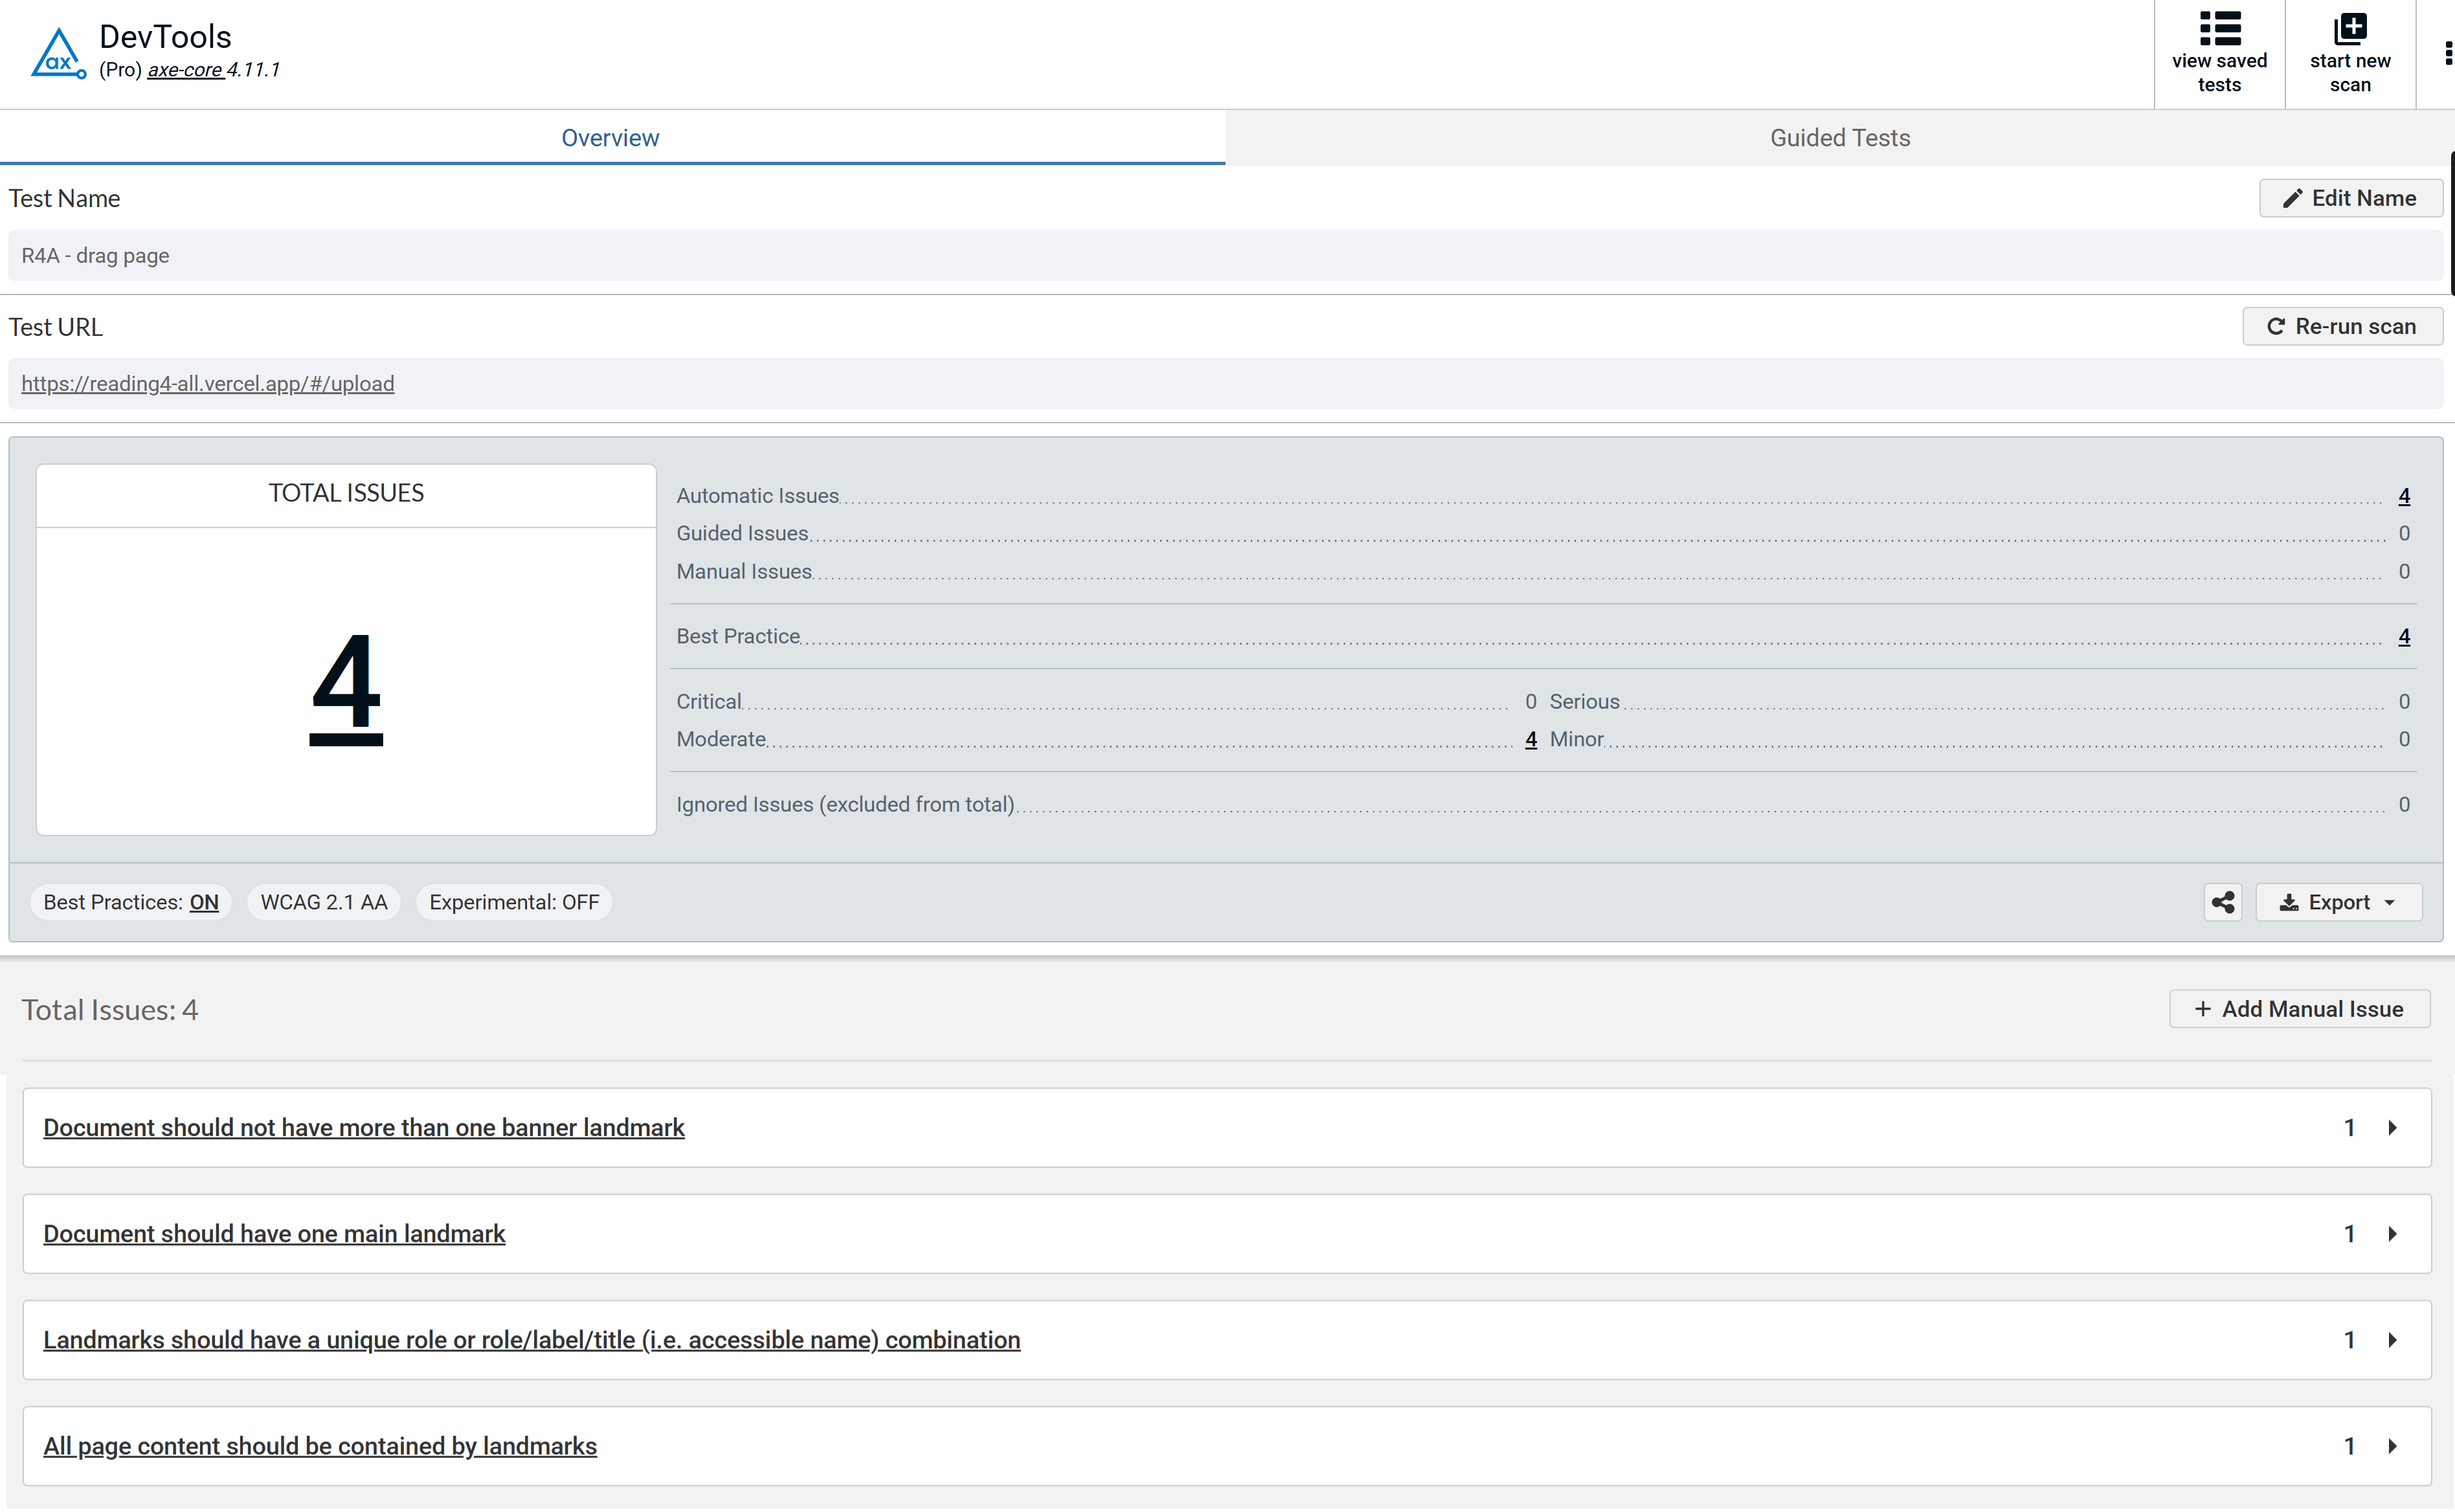
\includegraphics[width=\textwidth]{R4A_VnVRep_autoTest.png}
  \caption{Automated Report for ``Upload Page'' in the Reading4All System}
  \label{fig:work-context}
\end{figure}

Reports like these made it easier for the team to identify
accessibility oversights and best practices we might have missed and fix them.
Table~\ref{tab:axe-results} summarizes the Axe audit findings across the three main application pages.

\begin{table}[H]
\centering
\caption{Summary of Axe Accessibility Audit Results by Page}
\label{tab:axe-results}
\small
\begin{tabularx}{\textwidth}{|l|c|c|c|X|}
\hline
\textbf{Page} & \textbf{Critical} & \textbf{Serious} & \textbf{Moderate} & \textbf{Notes} \\
\hline
Login / Signup  & 0 & 0 & 1 & Missing \texttt{autocomplete} attribute on password field \\
\hline
Upload (Main)   & 0 & 1 & 2 & Missing \texttt{<main>} landmark (serious); duplicate \texttt{id} on rendered list items (moderate) \\
\hline
History         & 0 & 0 & 1 & Image previews lack \texttt{alt} attribute in some dynamic renders \\
\hline
\textbf{Total}  & \textbf{0} & \textbf{1} & \textbf{4} & No critical violations detected \\
\hline
\end{tabularx}
\end{table}

\noindent The missing \texttt{<main>} landmark (Upload page, serious) has since been corrected as described in the analysis of NFR-ST22. The remaining moderate issues are tracked as known defects for the next release. No critical or serious violations remain in the most recent build.

\subsection{CI/CD}

Continuous Integration and Continuous Deployment (CI/CD) practices
were used to ensure that changes to the Reading4All system could be
integrated and tested efficiently. Whenever updates were pushed to
the repository, automated workflows were triggered to verify that the
system built successfully and that core components continued to
function as expected.

These automated checks helped the team detect issues early in the
development process and prevented unstable code from being merged
into the main branch. By incorporating CI/CD into the development
workflow, Team 22 was able to maintain code quality, streamline
collaboration, and ensure that new features or fixes did not
unintentionally break existing functionality.

Additionally, the CI/CD pipeline supported reproducibility by
ensuring that the same build and testing procedures were executed
consistently for each update. This contributed to a more stable and
reliable development process for the Reading4All system.

\subsection{Mutation Testing}
Mutation testing was originally proposed in the VnV Plan as a method
to evaluate the effectiveness of unit tests by introducing small
faults (mutations) into the code and verifying whether the existing
tests could detect them. \\

However, mutation testing was not fully implemented in this project
due to time constraints and the additional setup complexity required
for integrating mutation testing tools with both the React frontend
and Python backend environments.
Additionally, the team prioritized functional correctness,
accessibility testing, and integration validation, which were more
critical to the system’s goals. \\

Despite not conducting formal mutation testing, test effectiveness
was indirectly assessed through code coverage analysis and the
ability of unit tests to detect real defects during development.
Future work could include incorporating
mutation testing tools to further evaluate and strengthen the
robustness of the test suite.

\section{Trace to Requirements}
The following table (Table \ref{table:test-requirement-trace}) shows
the relationship between the tests performed and
the requirements defined in the \citet{SRS}.\\
\noindent Note: Each test ID range maps to the SRS requirements it validates. For a matrix-style view showing individual test-to-requirement coverage, see Appendix~\ref{app:trace-matrix}.

\begin{table}[H]
  \centering
  \caption{Traceability Between Tests and Requirements}
  \label{table:test-requirement-trace}
  \small
  \begin{tabularx}{0.96\textwidth}{|>{\centering\arraybackslash}p{0.27\textwidth}|X|}
    \hline
    \textbf{Test ID} & \textbf{SRS Requirement(s) Satisfied} \\ \hline

    IMGVAL-UT1 -- IMGVAL-UT5 & FR 1, MD-SL 3, SR-IM 1 \\ \hline

    BCONT-UT1 -- BCONT-UT4 & FR 1, FR 2, FR 4, FR 5 \\ \hline

    AUTH-UT1 -- AUTH-UT6 & FR 6, SR-AR 1, SR-IM 2 \\ \hline

    MAIN-UT1 -- MAIN-UT18 & FR 1, FR 2, FR 4, UHR-EUR 1, UHR-EUR 2 \\ \hline

    HIST-UT1 -- HIST-UT4 & FR 5, UHR-EUR 2 \\ \hline

    LOGIN-UT1 -- LOGIN-UT16 & FR 6, SR-AR 1, SR-PR 1 \\ \hline

    UII-MT1 -- UII-MT6 & FR 1, FR 2, FR 4, FR 6, UHR-PIR 1 \\ \hline

    UIA-MT1 -- UIA-MT4 & LFR-AR 1, LFR-AR 3, LFR-AR 4, UHR-AR 2 \\ \hline

    DPP-MT1 -- DPP-MT4 & PR-SL 1, PR-SL 2, PR-PAR 1 \\ \hline

    MO-MT1 & FR 2, PR-PAR 2 \\ \hline

    AI-MT1 & PR-PAR 3 \\ \hline

    CG-MT1 & FR 2, PR-PAR 1 \\ \hline

    IMC-MT1 & PR-PAR 1, PR-PAR 2, PR-PAR 3 \\ \hline

    FR-ST1 -- FR-ST7 & FR 1 -- FR 6 \\ \hline

    NFR-ST1 -- NFR-ST26 & LFR-AR 1 -- LFR-AR 4, UHR-EUR 1 -- UHR-EUR 4, PR-SL 1 -- PR-SL 2, SR-AR 1, SR-PR 1, OER 1 \\ \hline

  \end{tabularx}
\end{table}

\section{Trace to Modules}

The following table (Table \ref{table:test-module-trace}) shows the
relationship between the tests performed
and the modules defined in the Module Guide. Each test verifies the
correct functionality of the corresponding module in the Reading4All system.
\noindent Note: Each test ID range maps to the SRS requirements it validates. For a matrix-style view showing individual test-to-requirement coverage, see Appendix~\ref{app:trace-matrix}.

\begin{table}[H]
  \centering
  \caption{Traceability Between Tests and Modules}
  \label{table:test-module-trace}
  \small
  \begin{tabularx}{0.96\textwidth}{|>{\centering\arraybackslash}p{0.27\textwidth}|X|}
    \hline
    \textbf{Test ID} & \textbf{Module} \\ \hline

    IMGVAL-UT1 -- IMGVAL-UT5 & ImageValidation Module \\ \hline
    BCONT-UT1 -- BCONT-UT4 & BackendController Module \\ \hline
    AUTH-UT1 -- AUTH-UT6 & AuthenticationService Module \\ \hline

    MAIN-UT1 -- MAIN-UT18 & MainScreen Module \\ \hline
    HIST-UT1 -- HIST-UT4 & ShowHistory Module \\ \hline
    LOGIN-UT1 -- LOGIN-UT16 & LoginScreen Module \\ \hline

    UII-MT1 -- UII-MT6 & UserInterfaceInteractions Module \\ \hline
    UIA-MT1 -- UIA-MT4 & UserInterfaceAccessibility Module \\ \hline

    DPP-MT1 -- DPP-MT4 & DataPreProcess Module \\ \hline

    MO-MT1 & ModelOutput Module \\ \hline
    AI-MT1 & AIModelTraining Module \\ \hline
    CG-MT1 & CaptionGeneration Module \\ \hline
    IMC-MT1 & InternalMetricCompliance Module \\ \hline

    FR-ST1 -- FR-ST7 & System Functional Tests (cross-module
    verification) \\ \hline
    NFR-ST1 -- NFR-ST26 & System Nonfunctional Tests (cross-module verification) \\ \hline

  \end{tabularx}
\end{table}

\section{Code Coverage Metrics}

The following analyzes the code coverage metrics for the React
frontend of the system. The analysis is based on the coverage data
generated using Jest and React Testing Library as shown in
Figure~\ref{fig:FrontendCoverage}. Code coverage is a measure of how
well the codebase is tested, and it helps identify areas that may
require additional testing.

\begin{figure}[H]
  \centering
  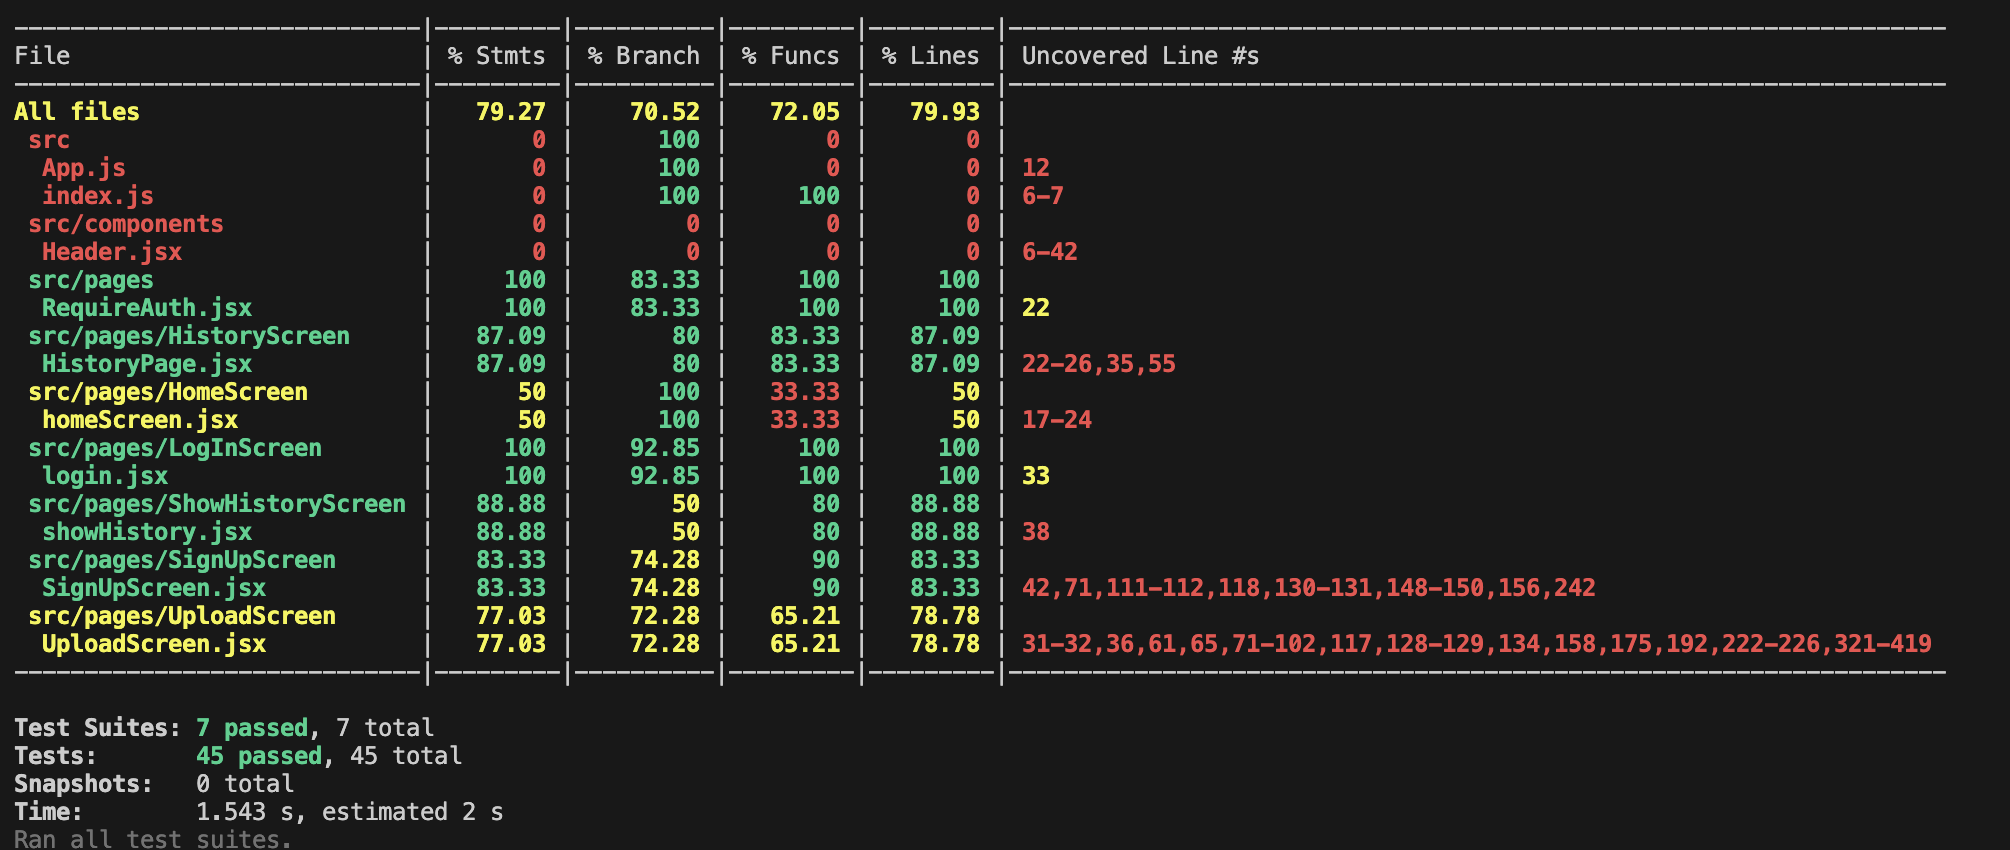
\includegraphics[width=0.8\textwidth]{FrontendCoverage.png}
  \caption{Coverage Report of the React Frontend}
  \label{fig:FrontendCoverage}
\end{figure}

The following analyzes the code coverage for the backend of the system.
This analysis was performed using \texttt{pytest-cov} and shows how key features
such as authentication, image validation, session history of the
system are unit tested.
Furthermore, files such as \texttt{alt\_text\_history.py} and
\texttt{gen\_alt\_text.py}
have lower unit test coverage due to their reliance on Supabase
database services. As a result,
their functionality was additionally tested manually to ensure correct
integration with Supabase and to ensure the expected behavior. Please
refer to the Figure~\ref{fig:BackendCoverage} for more detail and insight.

\begin{figure}[H]
  \centering
  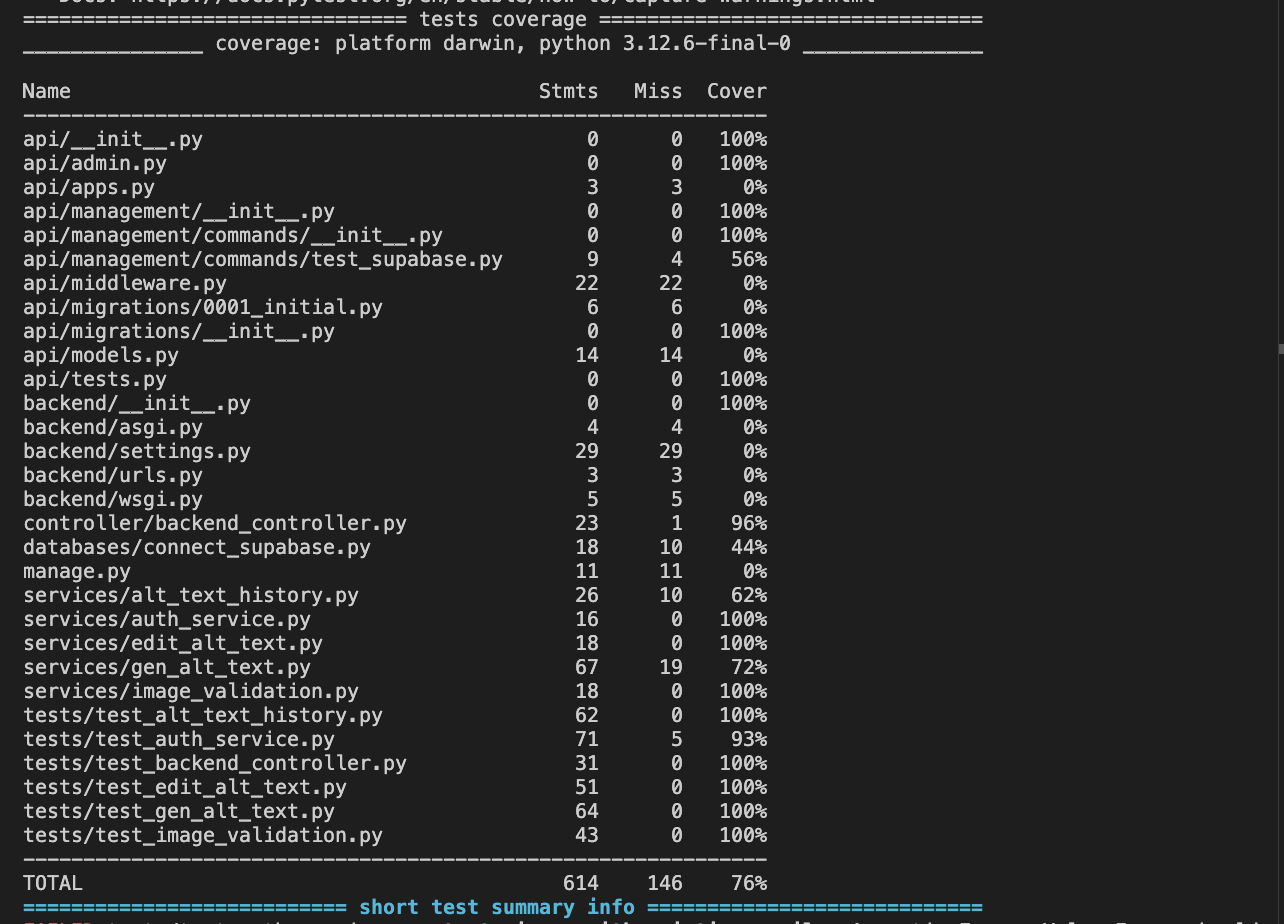
\includegraphics[width=1.1 \textwidth]{BackendCoverage_Updated.png}
  \caption{Coverage Report of the Backend}
  \label{fig:BackendCoverage}
\end{figure}

\bibliographystyle{plainnat}
\bibliography{../../refs/References}

\newpage{}
\section*{Appendix --- Traceability Matrix}
\label{app:trace-matrix}

Table~\ref{table:trace-matrix} provides a condensed matrix mapping selected test IDs to key functional and non-functional requirements.

\begin{table}[H]
\centering
\caption{Test-to-Requirement Traceability Matrix (Selected Tests)}
\label{table:trace-matrix}
\small
\begin{tabular}{|l|c|c|c|c|c|c|c|}
\hline
\textbf{Test ID} & \textbf{FR1} & \textbf{FR2} & \textbf{FR4} & \textbf{FR5} & \textbf{FR6} & \textbf{LFR-AR1} & \textbf{SR-AR1} \\
\hline
FR-ST1  & $\checkmark$ & & & & & & \\
FR-ST2  & & $\checkmark$ & & & & & \\
FR-ST3  & & $\checkmark$ & & & & $\checkmark$ & \\
FR-ST4  & & & $\checkmark$ & & & & \\
FR-ST5  & & & & $\checkmark$ & & & \\
FR-ST6  & & & & & $\checkmark$ & & $\checkmark$ \\
FR-ST7  & & & & & $\checkmark$ & & $\checkmark$ \\
NFR-ST1 & & & & & & $\checkmark$ & \\
NFR-ST5 & & $\checkmark$ & & & & $\checkmark$ & \\
NFR-ST12 & & & & & $\checkmark$ & & $\checkmark$ \\
\hline
\end{tabular}
\end{table}
\newpage{}
\section*{Appendix --- Reflection}

The information in this section will be used to evaluate the team members on the
graduate attribute of Reflection.

\input{../Reflection.tex}
None.

\textbf{Team Reflection}
\begin{enumerate}
  \item Which parts of this document stemmed from speaking to your client(s) or
    a proxy (e.g. your peers)? Which ones were not, and why?

    One aspect that stemmed from speaking with our supervisor is the
    importance of manual testing over automated testing, specifically
    the user interface.
    Our supervisor emphasized the importance of ensuring our
    interface is accessible and this is highlighted through our
    various nun-functional tests.
    We tried our best to put ourselves in the users shoes and
    understand any difficulties or issues they might face while using
    the Reading4All application.
    Furthermore, determining which aspects of the system to unit test
    verses manually test was determined through discussions with our
    TA supervisor. This was an aspect
    we were initialling unsure about; however, after discussions we
    determined that certain aspects such as the system as a whole,
    the accessibility, and alt text generation might be better manually tested.
    The Reading4All system implementation was mainly derived from our
    previous learnings through courses and industry standards, rather
    than from our clients and peers.

  \item In what ways was the Verification and Validation (VnV) Plan different
    from the activities that were actually conducted for VnV?  If there were
    differences, what changes required the modification in the plan?  Why did
    these changes occur?  Would you be able to anticipate these
    changes in future
    projects?  If there weren't any differences, how was your team
    able to clearly
    predict a feasible amount of effort and the right tasks needed to build the
    evidence that demonstrates the required quality?  (It is expected that most
    teams will have had to deviate from their original VnV Plan.)

    One way that the VnV plan was different from the activities
    conducted was that we initially planned to test all our modules,
    prior to us determining and forming our modules.
    This caused an issue when trying to actually conduct the VnV, as
    the modules were designed without having the testing in mind.
    This led us to have modules that were difficult
    to directly test and have concrete results for. As a result, one
    modification to the plan and overall system, is that certain
    modules had to be refactored as they could not be
    effectively tested and did not have any code we can point to.
    Furthermore, our VnV plan was dependent on a specific solution,
    that was vastly modified throughout the year. The VnV plan should
    have been written in a more
    generalized manner such that it would be flexible for any
    solution. For example, earlier in the year our team thought that
    a feedback module would be an appropriate way to train
    our AI model, however, through more research and various
    experiments, we determined that hypertuning would lead to better
    results. We believe we could not have anticipated this, as based
    on our AI knowledge at the time, we believed this would lead to
    the best design and implementation. Looking back, it's important
    for us to make a testing plan that depends more on the results
    and functionality that our system will exhibit rather than how it
    will be implemented as this often changes.

\end{enumerate}

\textbf{Fiza's Reflection}

\begin{enumerate}
  \item What went well while writing this deliverable?

    One aspect that went well while writing this deliverable was the
    clear structure provided by the VnV template and the previous
    planning documents. Since the system architecture, modules, and
    test plans were already defined in earlier deliverables such as
    the Module Guide and VnV Plan, it was easier to connect the
    implemented tests to the system components.
    Collaboration within the team also worked well, as each member
    was responsible for specific modules and testing sections, which
    allowed the work to be divided efficiently and integrated into a
    consistent report format.

  \item What pain points did you experience during this deliverable, and how
    did you resolve them?

    One challenge during this deliverable was ensuring consistency
    between the different sections of the report, such as aligning
    manual tests, system tests, and module traceability with the
    modules defined in the Module Guide. Another difficulty was
    formatting complex LaTeX tables and ensuring they compiled
    correctly while maintaining a consistent style across the
    document. These issues were resolved through iterative debugging
    of the LaTeX code and by coordinating with teammates to ensure
    the testing sections aligned with the previously defined modules
    and test cases.

\end{enumerate}

\textbf{Moly Mikhail's Reflection}

\begin{enumerate}
  \item What went well while writing this deliverable?

    I think many aspects went well while writing this deliverable.
    Writing the unit tests for the backend was a smooth process as
    I was highly familiar with the code base and the different
    branches to be covered. Another aspect that went well was
    documenting our unit test results, this also provided another
    opportunity for me to review the unit
    tests so far and to determine if any tests were missing and add them.

  \item What pain points did you experience during this deliverable, and how
    did you resolve them?

    One pain point I experienced writing this deliverable is
    determining the difference between the unit test section and
    automated testing.
    At first I was confused on the difference; however, after
    discussing with our TA, it was clearly they are highly related.
    Furthermore, it was also difficult determining which aspects of
    the system should be uni tested, verses manual tested. This was
    also cleared up through
    discussions with Chris. We decided the for integration testing it
    would be more effective to do it manually rather than to implement Selenium.

\end{enumerate}

\textbf{Dhruv Sardana's Reflection}

\begin{enumerate}
  \item What went well while writing this deliverable?
    I was responsible for writing the frontend modules tests.
    It helped me understand how to set up tests in Jest and React
    Testing Library and how to run coverage.
    Additionally, it helped me identify gaps in the application that
    were uncovered through testing.

  \item What pain points did you experience during this deliverable, and how
    did you resolve them?

    The challenges I faced were mainly related to setting up the
    testing environment and writing tests for React components that
    involve asynchronous operations,
    such as mocking API calls. I resolved these issues by referring
    to documentation and examples for Jest and React Testing Library,
    to ensure that the tests were correctly structured and covered
    the necessary functionality. Also another major challenge was to
    understand how to split up unit tests by modules
\end{enumerate}

\textbf{Nawaal Fatima's Reflection}
\begin{enumerate}
  \item What went well while writing this deliverable?
    The team was better prepared to work together. We split the doc
    as per usual and got to work, updating each other as often as
    possible. Our communication was stronger with each other this time around.

  \item What pain points did you experience during this deliverable, and how
    did you resolve them?
    My VSCode decided to crash every time I tried to work with it, so
    I had to ask my teammates to make my edits for me which was
    really annoying :(
      The tests we wrote for the VnV Plan didn't accurately encompass
      the solution we ended up building. They seemed disconnected
      from the solution itself as some parts had vastly changed from
      how we thought we'd implement it. This was frustrating because
      we knew our product worked, we just couldn't show it based on a
      plan we made before we started coding.
  \end{enumerate}

  \textbf{Casey Francine Bulaclac's Reflection}

  \begin{enumerate}
    \item What went well while writing this deliverable? \\
      One aspect that went well while writing the Verification and
      Validation report was being able to directly test our
      implemented modules and observe
      the outcomes of the test cases. Running the tests allowed us to
      clearly see which tests passed and which failed, which helped
      us better understand the current
      performance of our tool. This process was valuable because it
      highlighted areas where the system was functioning correctly as
      well as areas that could be improved for Revision 1.
      Another positive aspect was conducting user testing. Gathering
      feedback from users helped us identify what parts of the tool
      were working well and which parts needed improvement.
      Seeing how users interacted with the system provided practical
      insight and helped validate whether the tool behaved as
      expected from a user perspective.

    \item What pain points did you experience during this deliverable, and how
      did you resolve them? \\
      One challenge we encountered was that some modules originally
      described in the design documentation were not fully
      implemented in the final system. Because of this, we could
      not create meaningful verification tests for those modules as
      originally planned. This required us to revisit the testing
      plan and modify the VnV report so that the test
      cases only covered modules that were actually implemented and testable.
      To resolve this issue, we updated the relevant documentation to
      ensure consistency across all project deliverables. This
      involved adjusting parts of the MIS and MG documents so that
      they accurately reflected the system that was ultimately
      implemented. Although this required additional revisions, it
      ensured that the documentation, design descriptions, and testing
      procedures were all aligned with the final state of the project.

  \end{enumerate}

  \end{document}
